\documentclass[10pt]{extarticle}

\usepackage[english]{babel}
\usepackage{graphicx}
\usepackage{framed}
\usepackage[normalem]{ulem}
\usepackage{indentfirst}
\usepackage{amsmath,amsthm,amssymb,amsfonts}
\usepackage{mathtools} % Wraparound amsmath. For fancy math typesetting
\usepackage[nointegrals]{wasysym} % nointegrals prevents wasysym from overwriting integral symbols from LaTeX and amsmath
\usepackage{bbm} % For extended bold and blackboard bold characters
\usepackage[italicdiff]{physics} % italicdiff causes derivatives to be rendered with italic d's instead of upright d's
\usepackage[T1]{fontenc}
\usepackage{xparse}
\usepackage{xstring}
% \usepackage{pifont} % For unusual symbols
% \usepackage{mathdots} % For unusual combinations of dots
\usepackage{wrapfig}
\usepackage{lmodern,mathrsfs}
\usepackage[inline,shortlabels]{enumitem}
\setlist{topsep=2pt,itemsep=2pt,parsep=0pt,partopsep=0pt}
\usepackage[table,dvipsnames]{xcolor}
\usepackage[utf8]{inputenc}
\usepackage{csquotes} % Must be loaded AFTER inputenc
\usepackage[a4paper,top=0.5in,bottom=0.2in,left=0.5in,right=0.5in,footskip=0.3in,includefoot]{geometry}
\usepackage[most]{tcolorbox}
\usepackage{tikz,tikz-3dplot,tikz-cd,tkz-tab,tkz-euclide,pgf,pgfplots}
\pgfplotsset{compat=newest}
% \usepackage{comment} % For commenting large blocks of text and math efficiently
% \usepackage{fancyvrb} % For custom verbatim environments
\usepackage{multicol}
\usepackage[bottom,multiple]{footmisc} % Ensures footnotes are at the bottom of the page, and separates footnotes by a comma if they are adjacent
% \usepackage[backend=bibtex,style=numeric]{biblatex}
% \renewcommand*{\finalnamedelim}{\addcomma\addspace} % Forces authors' names to be separated by comma, instead of "and"
% \addbibresource{bibliography}
\usepackage[colorlinks,linkcolor=.,citecolor=blue,urlcolor=violet]{hyperref}
\usepackage[nameinlink]{cleveref} % nameinlink ensures that the entire element is clickable in the pdf, not just the number

\usepackage{epigraph} 
\usepackage{quantikz}
\usepackage{rotating}
\usepackage[dvipsnames]{xcolor}
\usepackage{cancel}
\usepackage{pifont}

\newcommand{\remind}[1]{\textcolor{red}{\textbf{#1}}} % To remind me of unfinished work to fix later
\newcommand{\hide}[1]{} % To hide large blocks of code without using % symbols

% Same as \href, but the text appears in typewriter font and in a custom color
\newcommand{\Href}[3][red!50!black]{\href{#2}{\textcolor{#1}{\texttt{#3}}}}

\newcommand{\ep}{\varepsilon}
\newcommand{\vp}{\varphi}
\newcommand{\lam}{\lambda}
\newcommand{\Lam}{\Lambda}
\DeclareDocumentCommand\ip{ l m }{\braces#1{\langle}{\rangle}{#2}} % Inner product ⟨x,y⟩ (but only one argument is taken, so \ip{x,y} renders as ⟨x,y⟩)
\DeclareDocumentCommand\floor{ l m }{\braces#1{\lfloor}{\rfloor}{#2}} % Floor function ⌊x⌋
\DeclareDocumentCommand\ceil{ l m }{\braces#1{\lceil}{\rceil}{#2}} % Ceiling function ⌈x⌉

% Shortcuts for blackboard bold letters, e.g. \A outputs \mathbb{A}
\def\do#1{\csdef{#1}{\mathbb{#1}}}
\docsvlist{A,B,C,D,E,F,G,I,J,K,M,N,Q,R,T,U,V,W,X,Y,Z}
% \H is already defined as a 1-argument command, it places a double acute accent (hungarumlaut) on a character, e.g. \H{o} yields ő
% \L is already defined as the uppercase Ł (L with stroke)
% \O is already defined as the uppercase Ø (O with stroke)
% \P is already defined as the pilcrow ¶ (paragraph mark)
% \S is already defined as the section sign §

% Shortcuts for calligraphic letters, e.g. \As outputs \mathcal{A}
\def\do#1{\csdef{#1s}{\mathcal{#1}}}
\docsvlist{A,B,C,D,E,F,G,H,I,J,K,L,M,N,O,P,Q,R,S,T,U,V,W,X,Y,Z}

% Shortcuts for letters with a bar on top, e.g. \Abar outputs \overline{A}
\def\do#1{\csdef{#1bar}{\overline{#1}}}
\docsvlist{a,b,c,d,e,f,g,i,j,k,l,m,n,o,p,q,r,s,t,u,v,w,x,y,z,A,B,C,D,E,F,G,H,I,J,K,L,M,N,O,P,Q,R,S,T,U,V,W,X,Y,Z}
% \hbar is already defined as the symbol ℏ (reduced Planck constant)

% Shortcuts for boldface letters, e.g. \Ab outputs \textbf{A}
\def\do#1{\csdef{#1b}{\textbf{#1}}}
\docsvlist{a,b,c,d,e,f,g,h,i,j,k,l,m,n,o,q,r,t,u,w,x,y,z,A,B,C,D,E,F,G,H,I,J,K,L,M,N,O,P,Q,R,S,T,U,V,W,X,Y,Z}
% \pb is already defined (by the physics package) as a 2-argument command, denoting the anticommutator or Poisson bracket, e.g. \pb{A,B} yields {A,B}
% \sb is already defined in the LaTeX kernel. This is a fundamental LaTeX command, DO NOT overwrite it!
% \vb is already defined (by the physics package) as a 1-argument command, for boldface text, e.g. \vb{A} yields \textbf{A}

% Shortcuts for letters with a tilde on top, e.g. \Atil outputs \widetilde{A}
\def\do#1{\csdef{#1til}{\widetilde{#1}}}
\docsvlist{a,b,c,d,e,f,g,h,i,j,k,l,m,n,o,p,q,r,s,t,u,v,w,x,y,z,A,B,C,D,E,F,G,H,I,J,K,L,M,N,O,P,Q,R,S,T,U,V,W,X,Y,Z}

\newcommand{\tm}{^{\mathsf{T}}}     % Transpose
\newcommand{\hm}{^{\mathsf{H}}}     % Conjugate transpose (Hermitian conjugate)
\newcommand{\itm}{^{-\mathsf{T}}}   % Inverse transpose
\newcommand{\ihm}{^{-\mathsf{H}}}   % Inverse conjugate transpose (Inverse Hermitian conjugate)
\newcommand{\ex}{\textbf{e}_x}
\newcommand{\ey}{\textbf{e}_y}
\newcommand{\ez}{\textbf{e}_z}
\newcommand{\Aint}{A^\circ}
\newcommand{\Bint}{B^\circ}
\newcommand{\limk}{\lim_{k\to\infty}}
\newcommand{\limm}{\lim_{m\to\infty}}
\newcommand{\limn}{\lim_{n\to\infty}}
\newcommand{\limx}[1][a]{\lim_{x\to#1}}
\newcommand{\limz}[1][{z_0}]{\lim_{z\to#1}}
\newcommand{\liminfm}{\liminf_{m\to\infty}}
\newcommand{\limsupm}{\limsup_{m\to\infty}}
\newcommand{\liminfn}{\liminf_{n\to\infty}}
\newcommand{\limsupn}{\limsup_{n\to\infty}}
\newcommand{\sumkn}{\sum_{k=1}^n}
\newcommand{\sumk}[1][1]{\sum_{k=#1}^\infty}
\newcommand{\summ}[1][1]{\sum_{m=#1}^\infty}
\newcommand{\sumn}[1][1]{\sum_{n=#1}^\infty}
\newcommand{\emp}{\varnothing}
\newcommand{\exc}{\backslash}
\newcommand{\sub}{\subseteq}
\newcommand{\sups}{\supseteq}
\newcommand{\capp}{\bigcap}
\newcommand{\cupp}{\bigcup}
\newcommand{\kupp}{\bigsqcup}
\newcommand{\cappkn}{\bigcap_{k=1}^n}
\newcommand{\cuppkn}{\bigcup_{k=1}^n}
\newcommand{\kuppkn}{\bigsqcup_{k=1}^n}
\newcommand{\cappk}[1][1]{\bigcap_{k=#1}^\infty}
\newcommand{\cuppk}[1][1]{\bigcup_{k=#1}^\infty}
\newcommand{\cappm}[1][1]{\bigcap_{m=#1}^\infty}
\newcommand{\cuppm}[1][1]{\bigcup_{m=#1}^\infty}
\newcommand{\cappn}[1][1]{\bigcap_{n=#1}^\infty}
\newcommand{\cuppn}[1][1]{\bigcup_{n=#1}^\infty}
\newcommand{\kuppk}[1][1]{\bigsqcup_{k=#1}^\infty}
\newcommand{\kuppm}[1][1]{\bigsqcup_{m=#1}^\infty}
\newcommand{\kuppn}[1][1]{\bigsqcup_{n=#1}^\infty}
\newcommand{\cappa}{\bigcap_{\alpha\in I}}
\newcommand{\cuppa}{\bigcup_{\alpha\in I}}
\newcommand{\kuppa}{\bigsqcup_{\alpha\in I}}
\newcommand{\dx}{\,dx}
\newcommand{\dy}{\,dy}
\newcommand{\dt}{\,dt}
\newcommand{\dmu}{\,d\mu}
\newcommand{\dnu}{\,d\nu}
\DeclareMathOperator{\glb}{\text{glb}}
\DeclareMathOperator{\lub}{\text{lub}}
\newcommand{\xh}{\widehat{x}}
\newcommand{\yh}{\widehat{y}}
\newcommand{\zh}{\widehat{z}}
\newcommand{\<}{\langle}
\renewcommand{\>}{\rangle}
% Colorful cancellations
\newcommand\ccancel[2][black]{\renewcommand\CancelColor{\color{#1}}\cancel{#2}}

% Shortcuts for inverse hyperbolic functions (and other operators with the same structure)
\def\do#1{\csdef{#1}{\trigbraces{\operatorname{#1}}}}
\docsvlist{
    asinh,acosh,atanh,acoth,asech,acsch,
    arsinh,arcosh,artanh,arcoth,arsech,arcsch,
    arcsinh,arccosh,arctanh,arccoth,arcsech,arccsch,
    sen,tg,cth,senh,tgh,ctgh,
    Re,Im,arg,Arg,im,ker
}

% \spn has to be defined separately as the syntax "spn" is different from the output "span"
% \span is already defined in the LaTeX kernel. This is a fundamental LaTeX command, DO NOT overwrite it!
\newcommand{\spn}{\trigbraces{\operatorname{span}}}

\makeatletter
% Redefining the commands \iff (given by LaTeX), \implies and \impliedby (given by amsmath)
% Math mode is automatically enforced, starred version makes the arrows shorter
\renewcommand{\impliedby}{\@ifstar{\ensuremath{\Longleftarrow}}{\ensuremath{\Leftarrow}}} % Corresponding Unicode character: U+21D0 ⇐
\renewcommand{\implies}{\@ifstar{\ensuremath{\Longrightarrow}}{\ensuremath{\Rightarrow}}} % Corresponding Unicode character: U+21D2 ⇒
\renewcommand{\iff}{\@ifstar{\ensuremath{\Longleftrightarrow}}{\ensuremath{\Leftrightarrow}}} % Corresponding Unicode character: U+21D4 ⇔
\makeatother

\newtheoremstyle{mystyle}{}{}{}{}{\sffamily\bfseries}{.}{ }{}
\makeatletter
\renewenvironment{proof}[1][Dowód] {\par\pushQED{\qed}{\normalfont\sffamily\bfseries\topsep6\p@\@plus6\p@\relax #1\@addpunct{.} }}{\popQED\endtrivlist\@endpefalse}
\makeatother
% \renewcommand{\qedsymbol}{\coolqed{0.32}} % Implements the new QED symbol
\theoremstyle{mystyle}{\newtheorem*{remark}{Obserwacja}}
\theoremstyle{mystyle}{\newtheorem*{remarks}{Obserwacje}}
\theoremstyle{mystyle}{\newtheorem*{example}{Przykład}}
\theoremstyle{mystyle}{\newtheorem*{examples}{Przykłady}}
\theoremstyle{definition}{\newtheorem*{exercise}{Ćwiczenie}}
\theoremstyle{mystyle}{\newtheorem*{fact}{Fakt}}
\theoremstyle{mystyle}{\newtheorem*{facts}{Fakty}}

% Warning environment
\newtheoremstyle{warn}{}{}{}{}{\normalfont}{}{ }{}
\theoremstyle{warn}
\newtheorem*{warning}{\warningsign{0.2}\relax}

% Symbol for the warning environment, designed to be easily scalable
\newcommand{\warningsign}[1]{
    \tikz[scale=#1,every node/.style={transform shape}]{
        \draw[-,line width={#1*0.8mm},red,fill=yellow,rounded corners={#1*2.5mm}] (0,0)--(1,{-sqrt(3)})--(-1,{-sqrt(3)})--cycle;
        \node at (0,-1) {\fontsize{48}{60}\selectfont\bfseries!};
}}

% \newcommand{\coolqed}[1]{\includegraphics[width=#1cm]{sunglasses_emoji.png}} % QED symbol

% verbbox environment, for showing verbatim text next to code output (for package documentation and user learning purposes)
\NewTCBListing{verbbox}{ !O{} }{boxrule=1pt,sidebyside,skin=bicolor,colback=gray!10,colbacklower=white,valign=center,top=2pt,bottom=2pt,left=2pt,right=2pt,#1} % Last argument allows more tcolorbox options to be added

\NewDocumentCommand{\solidball}{ s O{} m O{white} m }{
\tikz[scale=#5,every node/.style={transform shape}]{
    \shade[ball color=#3] (0,0) circle (0.5); %solid ball with no label
    \IfBooleanF{#1}{
        \clip (0,0) circle (0.25);
        \shade[ball color=#4] (0,0) circle (0.5);
    }
    \node[font=\sffamily\bfseries\selectfont] at (0,0) {#2}; % Label
}
}

\NewDocumentCommand{\stripedball}{ s O{} m O{white} m }{
\tikz[scale=#5,every node/.style={transform shape}]{
    \shade[ball color=#4] (0,0) circle (0.5);
    \clip (-0.5,-0.35) rectangle (0.5,0.35);
    \shade[ball color=#3] (0,0) circle (0.5);
    \IfBooleanF{#1}{
        \clip (0,0) circle (0.25);
        \shade[ball color=#4] (0,0) circle (0.5);
    }
    \node[font=\sffamily\bfseries\selectfont] at (0,0) {#2}; % Label
}
}

% Official colors for Aramith Tournament pool balls
% Colors taken from https://www.aramith.com/story-behind-aramith-tournament-black-colours
\definecolor{aramith_color_0}{HTML}{FFFFDF} % Cue ball and secondary color for all balls
\definecolor{aramith_color_1}{HTML}{FFD501} % 1 and 9
\definecolor{aramith_color_2}{HTML}{013CB1} % 2 and 10
\definecolor{aramith_color_3}{HTML}{E71C01} % 3 and 11
\definecolor{aramith_color_4}{HTML}{4F029C} % 4 and 12
\definecolor{aramith_color_5}{HTML}{FA4D00} % 5 and 13
\definecolor{aramith_color_6}{HTML}{0E5D01} % 6 and 14
\definecolor{aramith_color_7}{HTML}{6D071A} % 7 and 15
\definecolor{aramith_color_8}{HTML}{000000} % 8 (black)


\makeatletter
% Adapted from https://tex.stackexchange.com/a/61600
\csdef{aramith_pool_ball@0}#1{\solidball*{aramith_color_0}{#1}}                         % Cue ball
\csdef{aramith_pool_ball@1}#1{\solidball[1]{aramith_color_1}[aramith_color_0]{#1}}      % Ball 1
\csdef{aramith_pool_ball@2}#1{\solidball[2]{aramith_color_2}[aramith_color_0]{#1}}      % Ball 2
\csdef{aramith_pool_ball@3}#1{\solidball[3]{aramith_color_3}[aramith_color_0]{#1}}      % Ball 3
\csdef{aramith_pool_ball@4}#1{\solidball[4]{aramith_color_4}[aramith_color_0]{#1}}      % Ball 4
\csdef{aramith_pool_ball@5}#1{\solidball[5]{aramith_color_5}[aramith_color_0]{#1}}      % Ball 5
\csdef{aramith_pool_ball@6}#1{\solidball[6]{aramith_color_6}[aramith_color_0]{#1}}      % Ball 6
\csdef{aramith_pool_ball@7}#1{\solidball[7]{aramith_color_7}[aramith_color_0]{#1}}      % Ball 7
\csdef{aramith_pool_ball@8}#1{\solidball[8]{aramith_color_8}[aramith_color_0]{#1}}      % Ball 8 (black)
\csdef{aramith_pool_ball@9}#1{\stripedball[9]{aramith_color_1}[aramith_color_0]{#1}}    % Ball 9
\csdef{aramith_pool_ball@10}#1{\stripedball[10]{aramith_color_2}[aramith_color_0]{#1}}  % Ball 10
\csdef{aramith_pool_ball@11}#1{\stripedball[11]{aramith_color_3}[aramith_color_0]{#1}}  % Ball 11
\csdef{aramith_pool_ball@12}#1{\stripedball[12]{aramith_color_4}[aramith_color_0]{#1}}  % Ball 12
\csdef{aramith_pool_ball@13}#1{\stripedball[13]{aramith_color_5}[aramith_color_0]{#1}}  % Ball 13
\csdef{aramith_pool_ball@14}#1{\stripedball[14]{aramith_color_6}[aramith_color_0]{#1}}  % Ball 14
\csdef{aramith_pool_ball@15}#1{\stripedball[15]{aramith_color_7}[aramith_color_0]{#1}}  % Ball 15
\NewDocumentCommand{\poolball}{ o m m }{
    \pgfmathparse{Mod(#2,16)} % Argument #2 mod 16  as a floating-point number, e.g. 4.0
    \pgfmathtruncatemacro{\argumentmodulosixteen}{\pgfmathresult} % Convert to integer, e.g. 4.0 to 4
    \ifnum\argumentmodulosixteen=0
        \solidball*{aramith_color_0}{#3}
    \else
        \ifnum\argumentmodulosixteen<9
            \solidball[\IfNoValueTF{#1}{#2}{#1}]{aramith_color_\argumentmodulosixteen}[aramith_color_0]{#3} % Solid ball of the appropriate color, and the appropriate number (if the optional argument is not specified), otherwise the optional argument
        \else
            \pgfmathparse{\argumentmodulosixteen-8} % Argument #2 mod 8  as a floating-point number, e.g. 3.0 (this will only be computed if #2≥9)
            \pgfmathtruncatemacro{\argumentmoduloeight}{\pgfmathresult} % Convert to integer, e.g. 3.0 to 3
            \stripedball[\IfNoValueTF{#1}{#2}{#1}]{aramith_color_\argumentmoduloeight}[aramith_color_0]{#3} % Striped ball of the appropriate color, and the appropriate number (if the optional argument is not specified), otherwise the optional argument
        \fi
    \fi}
\makeatother

\makeatletter
% \fsize stores the current font size but is expandable (and can be called later without using \makeatletter and \makeatother)
\def\fsize{\dimexpr\f@size pt\relax}
\makeatother

\makeatletter
% Adapted from https://tex.stackexchange.com/a/19700
\def\my@vector #1,#2\@eolst{
    \ifx\relax#2\relax
        #1
    \else
        #1\my@delim
        \my@vector #2\@eolst
    \fi}
\newcommand\vcstring[2][\\]{% Converts comma-separated string to #1-separated string
    \def\my@delim{#1}
        \my@vector #2,\relax\noexpand\@eolst}
\newcommand\cvc[2][p]{% Converts comma-separated string to column vector, optional argument defines matrix brackets
    \def\my@delim{\\}
        \begin{#1matrix} % Empty argument also possible
            \my@vector #2,\relax\noexpand\@eolst
        \end{#1matrix}}
\newcommand\rvc[2][p]{% Converts comma-separated string to row vector, optional argument defines matrix brackets
    \def\my@delim{&}
        \begin{#1matrix} % Empty argument also possible
            \my@vector #2,\relax\noexpand\@eolst
        \end{#1matrix}}
% Matrix environment with variable number of arguments. Adapted from https://davidyat.es/2016/07/27/writing-a-latex-macro-that-takes-a-variable-number-of-arguments/
\newcommand{\mat}[2][p]{
    \def\matrixenvironment{#1matrix} % Specifying the matrix brackets, this has to be done beforehand as '#1' changes under \passtonextarg
    \def\my@delim{&}
        \begin{\matrixenvironment} % Begin matrix environment
            \my@vector #2,\relax\noexpand\@eolst
            \@ifnextchar\bgroup{\passtonextarg}{\end{\matrixenvironment}}% % Pass to next argument (if any), otherwise end matrix environment
}
\newcommand{\passtonextarg}[1]{\\ \my@vector #1,\relax\noexpand\@eolst
    \@ifnextchar\bgroup{\passtonextarg}{\end{\matrixenvironment}}% Passing to next argument
}
\makeatother

\definecolor{tcol_DEF}{HTML}{E40125} % Color for Definition
\definecolor{tcol_PRP}{HTML}{EB8407} % Color for Proposition
\definecolor{tcol_LEM}{HTML}{05C4D9} % Color for Lemma
\definecolor{tcol_THM}{HTML}{1346E4} % Color for Theorem
\definecolor{tcol_COR}{HTML}{7904C2} % Color for Corollary
\definecolor{tcol_REM}{HTML}{69A773} % Color for Remark
\definecolor{tcol_PRF}{HTML}{5A76B2} % Color for Proof
\definecolor{tcol_EXA}{HTML}{82A785} % Color for Example
\definecolor{tcol_FAC}{HTML}{D5F6FE} % Color for Fact


\tcbset{
tbox_DEF_style/.style={enhanced jigsaw,
    colback=tcol_DEF!10,colframe=tcol_DEF!80!black,
    fonttitle=\sffamily\bfseries,
    attach boxed title to top left={yshift=-\tcboxedtitleheight},
    boxed title style={
        boxrule=0pt,boxsep=2.5pt,
        colback=tcol_DEF!80!black,colframe=tcol_DEF!80!black,
        sharp corners=uphill
    },
    separator sign=.,label separator={},
    top=\tcboxedtitleheight,bottom=2pt,left=2pt,right=2pt,
    before skip=10pt,after skip=10pt,drop fuzzy shadow,breakable
},
tbox_PRP_style/.style={enhanced jigsaw,
    colback=tcol_PRP!10,colframe=tcol_PRP!80!black,
    fonttitle=\sffamily\bfseries,
    attach boxed title to top left={yshift=-\tcboxedtitleheight},
    boxed title style={
        boxrule=0pt,boxsep=2.5pt,
        colback=tcol_PRP!80!black,colframe=tcol_PRP!80!black,
        sharp corners=uphill
    },
    separator sign=.,label separator={},
    top=\tcboxedtitleheight,bottom=2pt,left=2pt,right=2pt,
    before skip=10pt,after skip=10pt,drop fuzzy shadow,breakable
},
tbox_PRB_style/.style={enhanced jigsaw,
    colback=tcol_PRP!10,colframe=tcol_PRP!80!black,
    fonttitle=\sffamily\bfseries,
    attach boxed title to top left={yshift=-\tcboxedtitleheight},
    boxed title style={
        boxrule=0pt,boxsep=2.5pt,
        colback=tcol_PRP!80!black,colframe=tcol_PRP!80!black,
        sharp corners=uphill
    },
    separator sign=.,label separator={},
    top=\tcboxedtitleheight,bottom=2pt,left=2pt,right=2pt,
    before skip=10pt,after skip=10pt,drop fuzzy shadow,breakable
},
tbox_THM_style/.style={enhanced jigsaw,
    colback=tcol_THM!10,colframe=tcol_THM!80!black,
    fonttitle=\sffamily\bfseries,
    attach boxed title to top left={yshift=-\tcboxedtitleheight},
    boxed title style={
        boxrule=0pt,boxsep=2.5pt,
        colback=tcol_THM!80!black,colframe=tcol_THM!80!black,
        sharp corners=uphill
    },
    separator sign=.,label separator={},
    top=\tcboxedtitleheight,bottom=2pt,left=2pt,right=2pt,
    before skip=10pt,after skip=10pt,drop fuzzy shadow,breakable
},
tbox_LEM_style/.style={enhanced jigsaw,
    colback=tcol_LEM!10,colframe=tcol_LEM!80!black,
    fonttitle=\sffamily\bfseries,
    attach boxed title to top left={yshift=-\tcboxedtitleheight},
    boxed title style={
        boxrule=0pt,boxsep=2.5pt,
        colback=tcol_LEM!80!black,colframe=tcol_LEM!80!black,
        sharp corners=uphill
    },
    separator sign=.,label separator={},
    top=\tcboxedtitleheight,bottom=2pt,left=2pt,right=2pt,
    before skip=10pt,after skip=10pt,drop fuzzy shadow,breakable
},
tbox_COR_style/.style={enhanced jigsaw,
    colback=tcol_COR!10,colframe=tcol_COR!80!black,
    boxrule=0pt,
    fonttitle=\sffamily\bfseries,coltitle=black,
    separator sign={},label separator={},
    description font=\normalfont\sffamily,
    description delimiters={(}{)},
    attach title to upper,after title={.\ },
    frame hidden,borderline west={2pt}{0pt}{tcol_COR},
    sharp corners,top=2pt,bottom=2pt,left=5pt,right=5pt,
    before skip=10pt,after skip=10pt,breakable
},
}

\newtcbtheorem[number within=section,
    crefname={\color{tcol_DEF!50!black} definition}{\color{tcol_DEF!50!black} definitions},
    Crefname={\color{tcol_DEF!50!black} Definition}{\color{tcol_DEF!50!black} Definitions}
    ]{definition}{Definicja}{tbox_DEF_style}{}
\newtcbtheorem[use counter from=definition,
    crefname={\color{tcol_PRP!50!black} proposition}{\color{tcol_PRP!50!black} propositions},
    Crefname={\color{tcol_PRP!50!black} Proposition}{\color{tcol_PRP!50!black} Propositions}
    ]{proposition}{Propozycja}{tbox_PRP_style}{}
\newtcbtheorem[use counter from=definition,
    crefname={\color{tcol_PRP!50!black} problem}{\color{tcol_PRP!50!black} problems},
    Crefname={\color{tcol_PRP!50!black} Problem}{\color{tcol_PRP!50!black} Problemy}
    ]{problem}{Problem}{tbox_PRB_style}{}
\newtcbtheorem[use counter from=definition,
    crefname={\color{tcol_THM!50!black} theorem}{\color{tcol_THM!50!black} theorems},
    Crefname={\color{tcol_THM!50!black} Theorem}{\color{tcol_THM!50!black} Theorems}
    ]{theorem}{Twierdzenie}{tbox_THM_style}{}
\newtcbtheorem[use counter from=definition,
    crefname={\color{tcol_LEM!50!black} lemma}{\color{tcol_LEM!50!black} lemmas},
    Crefname={\color{tcol_LEM!50!black} Lemma}{\color{tcol_LEM!50!black} Lemmas}
    ]{lemma}{Lemat}{tbox_LEM_style}{}
\newtcbtheorem[use counter from=definition,
    crefname={\color{tcol_COR!50!black} corollary}{\color{tcol_COR!50!black} corollaries},
    Crefname={\color{tcol_COR!50!black} Corollary}{\color{tcol_COR!50!black} Corollaries}
    ]{corollary}{Wniosek}{tbox_COR_style}{}

\makeatletter
\@namedef{tcolorboxshape@filingbox@ul}#1#2#3{
    (frame.south west)--(title.north west)--([xshift=-\dimexpr#1\relax]title.north east) to[out=0,in=180] ([xshift=\dimexpr#2\relax,yshift=\dimexpr#3\relax]title.south east)--(frame.north east)--(frame.south east)--cycle
}
\@namedef{tcolorboxshape@filingbox@uc}#1#2#3{
    (frame.south west)--(frame.north west)--([xshift=-\dimexpr#2\relax,yshift=\dimexpr#3\relax]title.south west) to[out=0,in=180] ([xshift=\dimexpr#1\relax]title.north west)--([xshift=-\dimexpr#1\relax]title.north east) to[out=0,in=180] ([xshift=\dimexpr#2\relax,yshift=\dimexpr#3\relax]title.south east)--(frame.north east)--(frame.south east)--cycle
}
\@namedef{tcolorboxshape@filingbox@ur}#1#2#3{
    (frame.south east)--(title.north east)--([xshift=\dimexpr#1\relax]title.north west) to[out=180,in=0] ([xshift=-\dimexpr#2\relax,yshift=\dimexpr#3\relax]title.south west)--(frame.north west)--(frame.south west)--cycle
}
\@namedef{tcolorboxshape@filingbox@dl}#1#2#3{
    (frame.north west)--(title.south west)--([xshift=-\dimexpr#1\relax]title.south east) to[out=0,in=180] ([xshift=\dimexpr#2\relax,yshift=-\dimexpr#3\relax]title.north east)--(frame.south east)--(frame.north east)--cycle
}
\@namedef{tcolorboxshape@filingbox@dc}#1#2#3{
    (frame.north west)--(frame.south west)--([xshift=-\dimexpr#2\relax,yshift=-\dimexpr#3\relax]title.north west) to[out=0,in=180] ([xshift=\dimexpr#1\relax]title.south west)--([xshift=-\dimexpr#1\relax]title.south east) to[out=0,in=180] ([xshift=\dimexpr#2\relax,yshift=-\dimexpr#3\relax]title.north east)--(frame.south east)--(frame.north east)--cycle
}
\@namedef{tcolorboxshape@filingbox@dr}#1#2#3{
    (frame.north east)--(title.south east)--([xshift=\dimexpr#1\relax]title.south west) to[out=180,in=0] ([xshift=-\dimexpr#2\relax,yshift=-\dimexpr#3\relax]title.north west)--(frame.south west)--(frame.north west)--cycle
}
\@namedef{tcolorboxshape@railingbox@ul}#1#2#3{
    (frame.south west)--(title.north west)--([xshift=-\dimexpr#1\relax]title.north east)--([xshift=\dimexpr#2\relax,yshift=\dimexpr#3\relax]title.south east)--(frame.north east)--(frame.south east)--cycle
}
\@namedef{tcolorboxshape@railingbox@uc}#1#2#3{
    (frame.south west)--(frame.north west)--([xshift=-\dimexpr#2\relax,yshift=\dimexpr#3\relax]title.south west)--([xshift=\dimexpr#1\relax]title.north west)--([xshift=-\dimexpr#1\relax]title.north east)--([xshift=\dimexpr#2\relax,yshift=\dimexpr#3\relax]title.south east)--(frame.north east)--(frame.south east)--cycle
}
\@namedef{tcolorboxshape@railingbox@ur}#1#2#3{
    (frame.south east)--(title.north east)--([xshift=\dimexpr#1\relax]title.north west)--([xshift=-\dimexpr#2\relax,yshift=\dimexpr#3\relax]title.south west)--(frame.north west)--(frame.south west)--cycle
}
\@namedef{tcolorboxshape@railingbox@dl}#1#2#3{
    (frame.north west)--(title.south west)--([xshift=-\dimexpr#1\relax]title.south east)--([xshift=\dimexpr#2\relax,yshift=-\dimexpr#3\relax]title.north east)--(frame.south east)--(frame.north east)--cycle
}
\@namedef{tcolorboxshape@railingbox@dc}#1#2#3{
    (frame.north west)--(frame.south west)--([xshift=-\dimexpr#2\relax,yshift=-\dimexpr#3\relax]title.north west)--([xshift=\dimexpr#1\relax]title.south west)--([xshift=-\dimexpr#1\relax]title.south east)--([xshift=\dimexpr#2\relax,yshift=-\dimexpr#3\relax]title.north east)--(frame.south east)--(frame.north east)--cycle
}
\@namedef{tcolorboxshape@railingbox@dr}#1#2#3{
    (frame.north east)--(title.south east)--([xshift=\dimexpr#1\relax]title.south west)--([xshift=-\dimexpr#2\relax,yshift=-\dimexpr#3\relax]title.north west)--(frame.south west)--(frame.north west)--cycle
}
\newcommand{\TColorBoxShape}[2]{\expandafter\ifx\csname tcolorboxshape@#1@#2\endcsname\relax
\expandafter\@gobble\else
\csname tcolorboxshape@#1@#2\expandafter\endcsname
\fi}
\makeatother

\tcbset{ % Styles for filingbox, railingbox and flagbox environments
% Adapted from https://tex.stackexchange.com/questions/587912/tcolorbox-custom-title-box-style
filingstyle/ul/.style 2 args={
    attach boxed title to top left={yshift=-2mm},
    boxed title style={empty,top=0mm,bottom=1mm,left=1mm,right=0mm},
    interior code={
        \path[fill=#1,rounded corners] \TColorBoxShape{filingbox}{ul}{9pt}{18pt}{6pt};
    },
    frame code={
        \path[draw=#2,line width=0.5mm,rounded corners] \TColorBoxShape{filingbox}{ul}{9pt}{18pt}{6pt};
    }},
filingstyle/uc/.style 2 args={
    attach boxed title to top center={yshift=-2mm},
    boxed title style={empty,top=0mm,bottom=1mm,left=0mm,right=0mm},
    interior code={
        \path[fill=#1,rounded corners] \TColorBoxShape{filingbox}{uc}{9pt}{18pt}{6pt};
    },
    frame code={
        \path[draw=#2,line width=0.5mm,rounded corners] \TColorBoxShape{filingbox}{uc}{9pt}{18pt}{6pt};
    }},
filingstyle/ur/.style 2 args={
    attach boxed title to top right={yshift=-2mm},
    boxed title style={empty,top=0mm,bottom=1mm,left=0mm,right=1mm},
    interior code={
        \path[fill=#1,rounded corners] \TColorBoxShape{filingbox}{ur}{9pt}{18pt}{6pt};
    },
    frame code={
        \path[draw=#2,line width=0.5mm,rounded corners] \TColorBoxShape{filingbox}{ur}{9pt}{18pt}{6pt};
    }},
filingstyle/dl/.style 2 args={
    attach boxed title to bottom left={yshift=2mm},
    boxed title style={empty,top=1mm,bottom=0mm,left=1mm,right=0mm},
    interior code={
        \path[fill=#1,rounded corners] \TColorBoxShape{filingbox}{dl}{9pt}{18pt}{6pt};
    },
    frame code={
        \path[draw=#2,line width=0.5mm,rounded corners] \TColorBoxShape{filingbox}{dl}{9pt}{18pt}{6pt};
    }},
filingstyle/dc/.style 2 args={
    attach boxed title to bottom center={yshift=2mm},
    boxed title style={empty,top=1mm,bottom=0mm,left=0mm,right=0mm},
    interior code={
        \path[fill=#1,rounded corners] \TColorBoxShape{filingbox}{dc}{9pt}{18pt}{6pt};
    },
    frame code={
        \path[draw=#2,line width=0.5mm,rounded corners] \TColorBoxShape{filingbox}{dc}{9pt}{18pt}{6pt};
    }},
filingstyle/dr/.style 2 args={
    attach boxed title to bottom right={yshift=2mm},
    boxed title style={empty,top=1mm,bottom=0mm,left=0mm,right=1mm},
    interior code={
        \path[fill=#1,rounded corners] \TColorBoxShape{filingbox}{dr}{9pt}{18pt}{6pt};
    },
    frame code={
        \path[draw=#2,line width=0.5mm,rounded corners] \TColorBoxShape{filingbox}{dr}{9pt}{18pt}{6pt};
    }},
railingstyle/ul/.style 2 args={
    attach boxed title to top left={yshift=-2mm},
    boxed title style={empty,top=0mm,bottom=1mm,left=1mm,right=0mm},
    interior code={
        \path[fill=#1] \TColorBoxShape{railingbox}{ul}{3pt}{12pt}{6pt};
    },
    frame code={
        \path[draw=#2,line width=0.5mm] \TColorBoxShape{railingbox}{ul}{3pt}{12pt}{6pt};
    }},
railingstyle/uc/.style 2 args={
    attach boxed title to top center={yshift=-2mm},
    boxed title style={empty,top=0mm,bottom=1mm,left=0mm,right=0mm},
    interior code={
        \path[fill=#1] \TColorBoxShape{railingbox}{uc}{3pt}{12pt}{6pt};
    },
    frame code={
        \path[draw=#2,line width=0.5mm] \TColorBoxShape{railingbox}{uc}{3pt}{12pt}{6pt};
    }},
railingstyle/ur/.style 2 args={
    attach boxed title to top right={yshift=-2mm},
    boxed title style={empty,top=0mm,bottom=1mm,left=0mm,right=1mm},
    interior code={
        \path[fill=#1] \TColorBoxShape{railingbox}{ur}{3pt}{12pt}{6pt};
    },
    frame code={
        \path[draw=#2,line width=0.5mm] \TColorBoxShape{railingbox}{ur}{3pt}{12pt}{6pt};
    }},
railingstyle/dl/.style 2 args={
    attach boxed title to bottom left={yshift=2mm},
    boxed title style={empty,top=1mm,bottom=0mm,left=1mm,right=0mm},
    interior code={
        \path[fill=#1] \TColorBoxShape{railingbox}{dl}{3pt}{12pt}{6pt};
    },
    frame code={
        \path[draw=#2,line width=0.5mm] \TColorBoxShape{railingbox}{dl}{3pt}{12pt}{6pt};
    }},
railingstyle/dc/.style 2 args={
    attach boxed title to bottom center={yshift=2mm},
    boxed title style={empty,top=1mm,bottom=0mm,left=0mm,right=0mm},
    interior code={
        \path[fill=#1] \TColorBoxShape{railingbox}{dc}{3pt}{12pt}{6pt};
    },
    frame code={
        \path[draw=#2,line width=0.5mm] \TColorBoxShape{railingbox}{dc}{3pt}{12pt}{6pt};
    }},
railingstyle/dr/.style 2 args={
    attach boxed title to bottom right={yshift=2mm},
    boxed title style={empty,top=1mm,bottom=0mm,left=0mm,right=1mm},
    interior code={
        \path[fill=#1] \TColorBoxShape{railingbox}{dr}{3pt}{12pt}{6pt};
    },
    frame code={
        \path[draw=#2,line width=0.5mm] \TColorBoxShape{railingbox}{dr}{3pt}{12pt}{6pt};
    }},
flagstyle/ul/.style 2 args={
    interior hidden,frame hidden,colbacktitle=#1,
    borderline west={1pt}{0pt}{#2},
    attach boxed title to top left={yshift=-8pt,yshifttext=-8pt},
    boxed title style={boxsep=3pt,boxrule=1pt,colframe=#2,sharp corners,left=4pt,right=4pt},
    bottom=0mm
    },
flagstyle/ur/.style 2 args={
    interior hidden,frame hidden,colbacktitle=#1,
    borderline east={1pt}{0pt}{#2},
    attach boxed title to top right={yshift=-8pt,yshifttext=-8pt},
    boxed title style={boxsep=3pt,boxrule=1pt,colframe=#2,sharp corners,left=4pt,right=4pt},
    bottom=0mm
    },
flagstyle/dl/.style 2 args={
    interior hidden,frame hidden,colbacktitle=#1,
    borderline west={1pt}{0pt}{#2},
    attach boxed title to bottom left={yshift=8pt,yshifttext=8pt},
    boxed title style={boxsep=3pt,boxrule=1pt,colframe=#2,sharp corners,left=4pt,right=4pt},
    top=0mm
    },
flagstyle/dr/.style 2 args={
    interior hidden,frame hidden,colbacktitle=#1,
    borderline east={1pt}{0pt}{#2},
    attach boxed title to bottom right={yshift=8pt,yshifttext=8pt},
    boxed title style={boxsep=3pt,boxrule=1pt,colframe=#2,sharp corners,left=4pt,right=4pt},
    top=0mm
    }
}

% Box in the shape of a filing divider, position of tab can be ul (up left), uc (up center), ur (up right), dl (down left), dc (down center) or dr (down right). Default is ul (upper left)
\NewTColorBox{filingbox}{ D(){ul} O{black} m O{} }{enhanced,
    top=1mm,bottom=1mm,left=1mm,right=1mm,
    title={#3},
    fonttitle=\sffamily\bfseries,
    coltitle=black,
    filingstyle/#1={#2!10}{#2},
    #4
}

% Box in the shape of a railing bar, position of tab can be ul (up left), uc (up center), ur (up right), dl (down left), dc (down center) or dr (down right). Default is ul (upper left)
\NewTColorBox{railingbox}{ D(){ul} O{black} m O{} }{enhanced,
    top=1mm,bottom=1mm,left=1mm,right=1mm,
    title={#3},
    fonttitle=\sffamily\bfseries,
    coltitle=black,
    railingstyle/#1={#2!10}{#2},
    #4
}

% Box in the shape of a flag, position of tab can be ul (up left), ur (up right), dl (down left) or dr (down right). Default is ul (upper left)
\NewTColorBox{flagbox}{ D(){ul} O{black} m O{} }{enhanced,breakable,
    top=1mm,bottom=1mm,left=1mm,right=1mm,
    title={#3},
    fonttitle=\sffamily\bfseries,
    coltitle=black,
    flagstyle/#1={#2!10}{#2},
    #4
}

\makeatletter
\newcommand*{\CreateSmartLargeOperator}[2]{
% Adapted from https://tex.stackexchange.com/questions/61598/new-command-with-cases-conditionals-if-thens/61600
    % Plain operator (no customization)
    \csdef{LargeOperator@#1@}{\csdef{LargeOperator@#1@Symbol}{\csuse{#1}}}
    % Operator with limits above and below symbol
    \csdef{LargeOperator@#1@l}{\csdef{LargeOperator@#1@Symbol}{\csuse{#1}\limits}}
    % Operato with limits beside symbol
    \csdef{LargeOperator@#1@n}{\csdef{LargeOperator@#1@Symbol}{\csuse{#1}\nolimits}}
    % Inline style operator
    \csdef{LargeOperator@#1@i}{\csdef{LargeOperator@#1@Symbol}{\textstyle\csuse{#1}}}
    % Display style operator
    \csdef{LargeOperator@#1@d}{\csdef{LargeOperator@#1@Symbol}{\displaystyle\csuse{#1}}}
    % Inline style operator with limits above and below symbol
    \csdef{LargeOperator@#1@il}{\csdef{LargeOperator@#1@Symbol}{\textstyle\csuse{#1}\limits}}
    % Inline style operator with limits beside symbol
    \csdef{LargeOperator@#1@in}{\csdef{LargeOperator@#1@Symbol}{\textstyle\csuse{#1}\nolimits}}
    % Display style operator with limits above and below symbol
    \csdef{LargeOperator@#1@dl}{\csdef{LargeOperator@#1@Symbol}{\displaystyle\csuse{#1}\limits}}
    % Display style operator with limits beside symbol
    \csdef{LargeOperator@#1@dn}{\csdef{LargeOperator@#1@Symbol}{\displaystyle\csuse{#1}\nolimits}}

% NOTE: In the command below, ##1 denotes the operator. It is NOT to be used as an argument!
\def\LargeOperatorSpecs@i##1,##2,##3,##4,##5,##6,##7\@nil{
% If no arguments, operate over n from 1 to infinity
    \ifx$##2$\csuse{LargeOperator@##1@Symbol}_{n=1}^{\infty}\else
    % If one argument, operate over n from ##2 to infinity
        \ifx$##3$\csuse{LargeOperator@##1@Symbol}_{n=##2}^{\infty}\else
        % If two arguments, operate over n from ##2 to ##3
            \ifx$##4$\csuse{LargeOperator@##1@Symbol}_{n=##2}^{##3}\else
            % If three arguments, operate over ##2 from ##3 to ##4
                \ifx$##5$\csuse{LargeOperator@##1@Symbol}_{##2=##3}^{##4}\else
                % If four arguments, operate over ##2 and ##3 from ##4 to ##5
                    \ifx$##6$\csuse{LargeOperator@##1@Symbol}_{##2,##3=##4}^{##5}\else
                    % If five arguments, operate over ##2, ##3 and ##4 from ##5 to ##6
                        \csuse{LargeOperator@##1@Symbol}_{##2,##3,##4=##5}^{##6}
                    \fi
                \fi
            \fi
        \fi
    \fi
}

% Flexible "smart" large operator macro with comma-separated arguments and optional argument for formatting. Default is over n from 1 to infinity. Adapted from https://tex.stackexchange.com/a/15722
\expandafter\DeclareDocumentCommand\csname#2\endcsname{ O{} m }{ % New operator macro
\bgroup % Group created to keep operator style (e.g. \limits) local
    \expandafter\ifx\csname LargeOperator@#1@##1\endcsname\relax
    \expandafter\@gobble\else
    \csname LargeOperator@#1@##1\expandafter\endcsname
    \fi
    \expandafter\LargeOperatorSpecs@i#1,##2,,,,,\@nil% % #1 stands in for the first "argument" of \LargeOperatorSpecs@i (the operator), the actual arguments are from ##2 onward
\egroup}
}
\makeatother

% Create the smart large operator #2 based on the large operator #1. For example, \CreateSmartLargeOperator{sum}{Sum} will define \Sum as the smart large operator based on \sum
% Equivalent Unicode characters are given here (but they are NOT the same as the operators)
\CreateSmartLargeOperator{sum}{Sum}             % Large: U+2211 ∑ (no small version)
\CreateSmartLargeOperator{prod}{Prod}           % Small: U+2293 ⊓, Large: U+220F ∏
\CreateSmartLargeOperator{coprod}{Coprod}       % Small: U+2294 ⊔, Large: U+2210 ∐
\CreateSmartLargeOperator{bigcap}{Capp}         % Small: U+2229 ∩, Large: U+22C2 ⋂
\CreateSmartLargeOperator{bigcup}{Cupp}         % Small: U+222A ∪, Large: U+22C3 ⋃
\CreateSmartLargeOperator{bigsqcup}{Kupp}       % Small: U+2294 ⊔, Large: U+2210 ∐
\CreateSmartLargeOperator{bigodot}{Odot}        % Small: U+2299 ⊙ (no large version)
\CreateSmartLargeOperator{bigoplus}{Oplus}      % Small: U+2295 ⊕ (no large version)
\CreateSmartLargeOperator{bigotimes}{Otimes}    % Small: U+2297 ⊗ (no large version)
\CreateSmartLargeOperator{biguplus}{Uplus}      % Small: U+228E ⊎ (no large version)
\CreateSmartLargeOperator{bigwedge}{Wedge}      % Small: U+2227 ∧, Large: U+22C0 ⋀
\CreateSmartLargeOperator{bigvee}{Vee}          % Small: U+2228 ∨, Large: U+22C1 ⋁

\tcolorboxenvironment{proof}{boxrule=0pt,boxsep=0pt,blanker,
    borderline west={2pt}{0pt}{tcol_PRF},left=8pt,right=8pt,sharp corners,
    before skip=10pt,after skip=10pt,breakable
}
\tcolorboxenvironment{remark}{boxrule=0pt,boxsep=0pt,blanker,
    borderline west={2pt}{0pt}{tcol_REM},left=8pt,right=8pt,
    before skip=10pt,after skip=10pt,breakable
}
\tcolorboxenvironment{remarks}{boxrule=0pt,boxsep=0pt,blanker,
    borderline west={2pt}{0pt}{tcol_REM},left=8pt,right=8pt,
    before skip=10pt,after skip=10pt,breakable
}
\tcolorboxenvironment{example}{boxrule=0pt,boxsep=0pt,blanker,
    borderline west={2pt}{0pt}{tcol_EXA},left=8pt,right=8pt,sharp corners,
    before skip=10pt,after skip=10pt,breakable
}
\tcolorboxenvironment{examples}{boxrule=0pt,boxsep=0pt,blanker,
    borderline west={2pt}{0pt}{tcol_EXA},left=8pt,right=8pt,sharp corners,
    before skip=10pt,after skip=10pt,breakable
}
\tcolorboxenvironment{fact}{boxrule=0pt,boxsep=0pt,blanker,
    borderline west={2pt}{0pt}{tcol_FAC},left=8pt,right=8pt,sharp corners,
    before skip=10pt,after skip=10pt,breakable
}
\tcolorboxenvironment{facts}{boxrule=0pt,boxsep=0pt,blanker,
    borderline west={2pt}{0pt}{tcol_FAC},left=8pt,right=8pt,sharp corners,
    before skip=10pt,after skip=10pt,breakable
}

% align and align* environments with inline size
\newenvironment{talign}{\let\displaystyle\textstyle\align}{\endalign}
\newenvironment{talign*}{\let\displaystyle\textstyle\csname align*\endcsname}{\endalign}

\usepackage[explicit]{titlesec}
% Setting the format for sections, subsections and subsubsections
\titleformat{\section}{\fontsize{24}{30}\sffamily\bfseries}{\thesection}{20pt}{#1}
\titleformat{\subsection}{\fontsize{16}{18}\sffamily\bfseries}{\thesubsection}{12pt}{#1}
\titleformat{\subsubsection}{\fontsize{10}{12}\sffamily\large\bfseries}{\thesubsubsection}{8pt}{#1}
% Setting the spacing for sections, subsections and subsubsections
% First argument is the left indent, second argument is the spacing above, third argument is the spacing below
\titlespacing*{\section}{0pt}{5pt}{5pt}
\titlespacing*{\subsection}{0pt}{5pt}{5pt}
\titlespacing*{\subsubsection}{0pt}{5pt}{5pt}

\newcommand{\Disp}{\displaystyle}
\newcommand{\qe}{\hfill\(\bigtriangledown\)}
\DeclareMathAlphabet\mathbfcal{OMS}{cmsy}{b}{n}
\setlength{\parindent}{0.2in}
\setlength{\parskip}{0pt}
\setlength{\columnseprule}{0pt}

\makeatletter
% Modify spacing above and below display equations
\g@addto@macro\normalsize{
    \setlength\abovedisplayskip{3pt}
    \setlength\belowdisplayskip{3pt}
    \setlength\abovedisplayshortskip{0pt}
    \setlength\belowdisplayshortskip{0pt}
}
\makeatother

\makeatletter
% Redefining the title block
\renewcommand\maketitle{
\null % \vspace does not work with nothing above it, so \null is added
\vspace{5mm}
\begingroup % Creating a group to ensure col_stripes is only defined locally, i.e. only for the title
\definecolor{col_stripes}{HTML}{1B0982} % Color of the stripes above and below the title components
    \begin{tcolorbox}[enhanced,blanker,
    borderline horizontal={2pt}{0pt}{col_stripes},
    borderline horizontal={1pt}{-3.5pt}{col_stripes},
    borderline horizontal={2pt}{-8pt}{col_stripes},
    fontupper=\fontfamily{bch},
    halign=flush center,top=10mm,bottom=10mm,after skip=20mm,
    ]
        {\fontsize{24}{28}\bfseries\selectfont\@title}\\
            \vspace{6mm}
        {\fontsize{20}{24}\selectfont\@author}\\
            \vspace{6mm}
        {\fontsize{16}{20}\selectfont\@date}
    \end{tcolorbox}
\endgroup}
% Adapted from https://tex.stackexchange.com/questions/483953/how-to-add-new-macros-like-author-without-editing-latex-ltx?noredirect=1&lq=1
\makeatother

\title{Kwanty}
\author{Jacek Markiewicz}
\date{2025/2026} % Replace with \today to show the current date

% Based on 'Fun Template 1', available at https://www.overleaf.com/latex/templates/fun-template-1/drwvdzsrpgzz

\begin{document}

\maketitle

\definecolor{tcol_CNT1}{HTML}{72E094} % First color for Contents
\definecolor{tcol_CNT2}{HTML}{24E2D6} % Second color for Contents
\definecolor{tcol_CNV1}{HTML}{8E44AD} % First color for Conventions
\definecolor{tcol_CNV2}{HTML}{A10B49} % First color for Conventions

\epigraph{Imagination will often carry us to worlds that never were. But without it we go nowhere.}{\textit{Carl Sagan}}

% \newpage

\begin{tcolorbox}[enhanced,
    title=Spis treści,
    fonttitle=\fontsize{20}{24}\sffamily\bfseries\selectfont,
    coltitle=black,
    fontupper=\sffamily,
    interior style={left color=tcol_CNT1!80,right color=tcol_CNT2!80},
    frame style={left color=tcol_CNT1!60!black,right color=tcol_CNT2!60!black},
    attach boxed title to top center={yshift=10pt},
    boxed title style={frame hidden,
        interior style={left color=tcol_CNT1,right color=tcol_CNT2},
        frame style={left color=tcol_CNT1!60!black,right color=tcol_CNT2!60!black},
        height=24pt,bean arc,drop fuzzy shadow
    },
    top=2mm,bottom=2mm,left=2mm,right=2mm,
    before skip=20mm,after skip=20mm,
    drop fuzzy shadow,breakable]
%
\makeatletter
\@starttoc{toc}
\makeatother
\end{tcolorbox}

% \begin{tcolorbox}[enhanced,
%     frame hidden,
%     title=Conventions,
%     fonttitle=\large\sffamily\bfseries\selectfont,
%     interior code={
%         \shade[top color=tcol_CNV2!50,bottom color=white] ([yshift=2mm]interior.north west) arc(-180:-90:2mm)--(interior.north east)--(interior.south east)--(interior.south west)--cycle;
%         },
%     overlay={
%         \draw[tcol_CNV1!50!black,line width=0.5mm] ([xshift=2mm]frame.north west)--(frame.north east);
%     },
%     boxrule=0pt,left=2pt,right=2pt,
%     sharp corners=north,
%     attach boxed title to top left,
%     boxed title style={interior hidden,
%     left=1mm,right=1mm,
%     frame code={
%         \path[draw=tcol_CNV1!50!black,line width=0.5mm,fill=tcol_CNV1,rounded corners=2mm] ([xshift=2mm]frame.south east)--(frame.south east)--(frame.north east)--([xshift=0.25mm]frame.north west)--([xshift=0.25mm]frame.south west)--cycle;}
%     },
%     top=2mm,bottom=2mm,left=2mm,right=2mm,
%     before skip=10mm,after skip=10mm]
% %
% $\F$ denotes either $\R$ or $\C$.\\
% $\N$ denotes the set $\{1,2,3,\ldots\}$ of natural numbers (excluding $0$).\\
% Inner products are taken to be linear in the first argument and conjugate linear in the second.\\
% The Einstein summation convention is used for tensors unless otherwise specified.
% \end{tcolorbox}

% ------------------------------------------------------------------------------------------
\newpage
\section{Wstęp}
\begin{definition*}{}
    Macierz $U$ jest \textbf{unitarna} gdy $UU^\dagger = U^\dagger U = I$. \\
    Macierz $U$ nazywamy \textbf{hermitowską} jeśli $U = U^\dagger$. 
\end{definition*}
Macierze unitarne są dla nas istotne o tyle, że bramki kwantowe są właśnie operatorami unitarnymi.
\begin{lemma*}{}
    Macierze unitarne zachowują normę $L_2$.
\end{lemma*}
\begin{proof}
    Niech $v$ to dowolny element taki, że $\norm{v}_2=1$. Poza tym niech $U$ - macierz unitarna, czyli $UU^\dagger = U\dagger U = I$. Wtedy: 
    \[ \norm{v}_2 = \braket{v}{v} = \bra{v}\cdot \ket{v} = \bra{v} \cdot I \cdot \ket{v} = \bra{v} \cdot (U^\dagger U) \cdot \ket{v} \]
    \[ = \Bigl(\bra{v}U^\dagger\Bigr)\Bigl(U\ket{v}\Bigr) = \Bigl(U\ket{v}\Bigr)^\dagger\Bigl(U\ket{v}\Bigr) = \braket{Uv}{Uv} = \norm{Uv}_2 \]
\end{proof}

\subsection{Stany Bella}
\begin{definition*}{}
    \textbf{Stanami Bella} określamy 2-kubitowe stany \( \frac{\ket{00} \pm \ket{11}}{\sqrt2} \) oraz \( \frac{\ket{01} \pm \ket{10}}{\sqrt2} \).   
\end{definition*}
Stany Bella są najprostszym przykładem splątania kwantowego. Zmierzenie wartości pierwszego kubitu sprawi, że wartość drugiego kubitu zostanie już ustalona. Jednak gdybyśmy nie zmierzyli pierwszego kubitu, to pomiar drugiego z nich mógłby wyprodukować zarówno $0$ jak i $1$. \\
Nietrudno stworzyć taki stan. Czyni to na przykład następujący układ:
\begin{align}
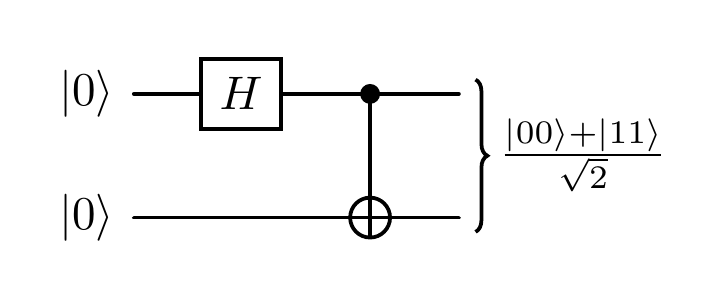
\begin{tikzpicture}
\node[scale=1.7]{
\begin{quantikz}
\lstick{$\ket{0}$} & \gate{H} & \ctrl{1} & \rstick[2]{$\frac{\ket{00}+\ket{11}}{\sqrt2}$}  \\
\lstick{$\ket{0}$} &          & \targ{}  &
\end{quantikz}
};
\end{tikzpicture}
\end{align}

Jest tak, bo:
\[ \ket{00} \xmapsto{H\otimes I} \Bigl(\frac{\ket{0}+\ket{1}}{\sqrt2}\Bigr)\ket{0} = \frac{\ket{00}+\ket{10}}{\sqrt2} \xmapsto{CX} \frac{\ket{00}+\ket{11}}{\sqrt2} \]


% ------------------------------------------------------------------------------------------
\newpage
\section{Algorytm Deutscha-Jozsy}
\begin{problem*}{} 
    Dana jest czarna skrzynka w postaci funkcji $f: \{0,1\}^n \rightarrow \{0,1\}$, o której wiemy, że zachodzi jedno z poniższych:
    \begin{itemize}
        \item $f$ jest funkcją \textit{stałą} (zawsze zwraca 0 lub zawsze zwraca 1) lub
        \item $f$ jest funkcją \textit{zbalansowaną} (przypisuje 0 takiej samej ilości elementów co wartość 1)
    \end{itemize}
    Naszym zadaniem jest stwierdzenie, czy $f$ jest stała czy zbalansowana. \\
    Chcemy dodatkowo dokonać tego wykonując możliwie mało ewaluacji funkcji $f$.
\end{problem*}

\subsection*{Klasyczne podejście}
    Na komputerze klasycznym konieczne jest $\Os(2^n)$ operacji. Wynika to z tego, że pesymistycznie pierwsze $2^{n-1}$ sprawdzeń wartości może zakończyć się tym samym wynikiem, niezależnie jakiego rodzaju jest to funkcja. \\

    Innym pomysłem jest algorytm randomizowany, tj. wylosowanie $k$ wartości i ich zewaluowanie. Jeśli otrzymaliśmy zarówno 0 jak i 1 jako wyniki, to funkcja na pewno była zbalansowana. Wpp. strzelamy, że była funkcją stałą. Jest to niezła metoda, gdyż prawdopodobieństwo pomyłki (czyli uznania $f$ za stałą gdy była tylko zbalansowaną) wynosi $2^{-k}$. Wymagało to dodatkowo tylko $k$ ewaluacji funkcji $f$. 

    \subsection*{Kwantowe podejście}
    My jednak będziemy jeszcze lepsi i stworzymy algorytm deteministyczny, który da nam zawsze poprawną odpowiedź wykonując tylko jedną ewaluację funkcji $f$. Bez owijania w bawełnę oto nasz szukany obwód kwantowy:
        
\begin{align}
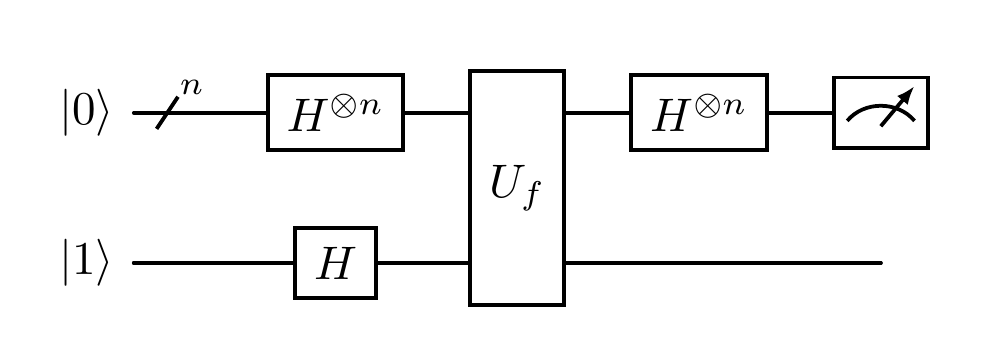
\begin{tikzpicture}
\node[scale=1.7]{
\begin{quantikz}
\lstick{$\ket{0}$} & \qwbundle{n} & \gate{H^{\otimes n}}  & \gate[2]{U_f}  & \gate{H^{\otimes n}} & \meter{} \\
\lstick{$\ket{1}$} & \qw & \gate{H} & \qw & \qw & \qw
\end{quantikz}
};
\end{tikzpicture}
\end{align}
Jeśli zmierzymy $\ket{0}^{\otimes n}$ to funkcja była stała. W przeciwnym przypadku była zbalansowana.

\begin{proof}

Żeby zobaczyć dlaczego ten układ rozwiązuje nasz problem musimy przeanalizować co się dzieje w każdym jego kroku:

\begin{align}
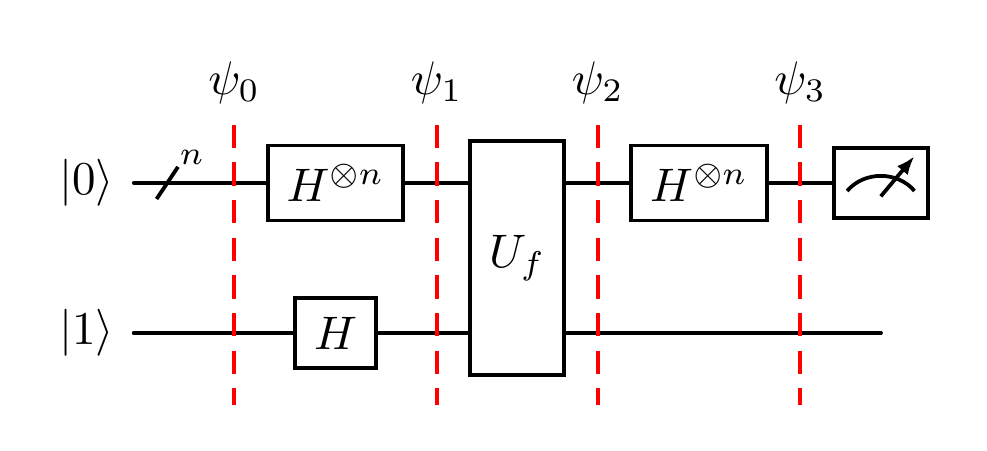
\begin{tikzpicture}
\node[scale=1.7]{
\begin{quantikz}
\lstick{$\ket{0}$} & \qwbundle{n}\slice{$\psi_0$} & \gate{H^{\otimes n}}\slice{$\psi_1$}  & \gate[2]{U_f}\slice{$\psi_2$}  & \gate{H^{\otimes n}}\slice{$\psi_3$} & \meter{} \\
\lstick{$\ket{1}$} & \qw & \gate{H} & \qw & \qw & \qw
\end{quantikz}
};
\end{tikzpicture}
\end{align}

\begin{itemize}
\item $\ket{\psi_0} = \ket{0^{\otimes n}}\ket{1}$
\item $\ket{\psi_1}$: \\ 
    Przypomnijmy sobie jak działa bramka Hadamarda:
    \[ H\ket{0}^{\otimes n} = \frac{1}{\sqrt{2^n}}\sum_{x=0}^{2^n-1}\ket{x} \]
    \[ H\ket{1} = \frac{1}{\sqrt{2}}\left(\ket{0}-\ket{1}\right) \]
    Podstawiając
    \[\ket{\psi_1} = H\ket{\psi_0} = (H\ket{0}^{\otimes n})(H\ket{1}) = \frac{1}{\sqrt{2^{n+1}}}\sum_{x=0}^{2^n-1}\ket{x}\left(\ket{0}-\ket{1}\right)  \]
\item $\ket{\psi_2}$: \\
    Wyrocznia $U_f$ zachowuje się tak:
    \[ U_f\ket{x}_n\ket{y} = \ket{x}_n\ket{y\oplus{f(x)}} \]
    
    \[ \Rightarrow  \ket{\psi_2} = U_f\ket{\psi_1} = \frac{1}{\sqrt{2^{n+1}}}\sum_{x=0}^{2^n-1}\ket{x}\left(\ket{f(x)}-\ket{1\oplus f(x)}\right) \]
    ale $f(x)$ przyjmuje tylko wartości 0 lub 1, zatem możemy zapisać to sprytniej
    \[ = \frac{1}{\sqrt{2^{n+1}}}\sum_{x=0}^{2^n-1} (-1)^{f(x)}\ket{x}\left(\ket{0}-\ket{1}\right) \]

\item $\ket{\psi_3}$: \\
    Bramka Hadamarda potrafi jeszcze tak:
        \[ H\ket{x} = \frac{1}{\sqrt{2^n}}\sum_{i=0}^{2^n-1}(-1)^{x\cdot i}\ket{i}\]
    gdzie $x\cdot i$ oznacza iloczyn skalarny, czyli $x\cdot i = x_1i_1 \oplus ... \oplus x_ni_n$. \\
    Ostatni wynikowy kubit nie jest nam potrzebny, więc go ignorujemy. Zatem niech $\psi_2'$ oznacza stan $\psi_2$ z uciętym ostatnim bitem, analogicznie $\psi_3'$. Wtedy:
    \[ \ket{\psi_2'} = \frac{1}{\sqrt{2^{n}}}\sum_{x=0}^{2^n-1} (-1)^{f(x)}\ket{x} \]
    Zatem ostatnia transformacja daje nam
    \[ \ket{\psi_3'} = H\ket{\psi_2'} = \frac{1}{2^n}\sum_{x=0}^{2^{n-1}}(-1)^{f(x)}\cdot \sum_{i=0}^{2^n-1}(-1)^{x\cdot i}\ket{i} \]
    \[ = \frac{1}{2^n} \sum_{i=0}^{2^n-1} \left[ \sum_{x=0}^{2^n-1}(-1)^{f(x)}(-1)^{x\cdot i} \right]\ket{i} \]
    Ale teraz zauważmy, że prawdopodobieństwo zmierzenia stanu $0^{\otimes n}$ wynosi
    \[ \left|\frac{1}{2^n}\sum_{x=0}^{2^n-1}(-1)^{f(x)} \right|^2 \]
    Wystarczy teraz przeanalizować przypadki:
    \begin{enumerate}
        \item Jeśli $f$ jest stała, to $\sum_{x=0}^{2^n-1} = \pm 2^n$, czyli prawdopodobieństwo wyjdzie równe 1.
        \item Jeśłi $f$ jest zbalansowana, to $\sum_{x=0}^{2^n-1} = 0$, bo wyrazów sumy równych 1 jest tyle samo co równych -1. Zatem prawdopodobieństwo wyniesie 0. 
    \end{enumerate}
    Czyli by stwierdzić czy $f$ jest stała wystarczy sprawdzić czy na końcu zmierzymy $0^{\otimes n}$. Jeśli zmierzymy cokolwiek innego to znaczy, że była zbalansowana.
\end{itemize}
\end{proof}

\subsection{Bernstein–Vazirani}
\begin{problem*}{}
    Dana jest czarna skrzynka w postaci funkcji $f: \{0,1\}^n\rightarrow\{0,1\}$. Mamy zapewnione, że $f$ jest postaci
    \[ f(x) = x\cdot s \]
    gdzie $\cdot$ jest iloczynem skalarnym $mod$ $2$, a $s$ - nieznanym wektorem z $\{0,1\}^n$. \\
    Zadanie polega na wyznaczeniu $s$. \\
    Dodatkowo chcemy tego dokonać wykonując możliwie mało zapytań o funkcję $f$.
\end{problem*}

Łatwo pokazać, że klasyczne podejście zawsze wymaga co najmniej $n$ zapytań o wartość $f(x)$. Wynika to z faktu, że przestrzeń potencjalnych wartości $s$ jest wielkości $2^n$, a każde zapytanie się o wartość $f(x)$ odrzuca pewną część tej przestrzeni, pesymistycznie co najwyżej połowę. Czyli aby być pewnym wartości $s$ trzeba wykonać co najmniej $\lg(2^n) = n$ zapytań. \\

My będziemy lepsi i wyznaczymy deterministycznie wartość $s$ używając tylko jednej ewaluacji funkcji $f$. \\
By to osiągnąć użyjemy następującego układu:

\begin{align}
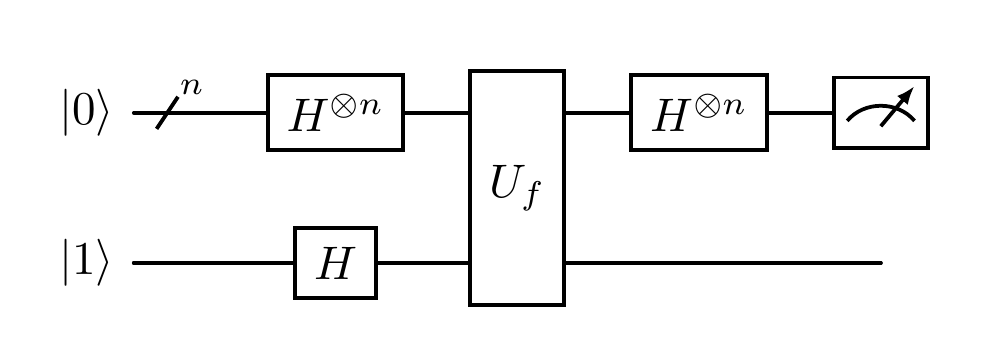
\begin{tikzpicture}
\node[scale=1.7]{
\begin{quantikz}
\lstick{$\ket{0}$} & \qwbundle{n} & \gate{H^{\otimes n}}  & \gate[2]{U_f}  & \gate{H^{\otimes n}} & \meter{} \\
\lstick{$\ket{1}$} & \qw & \gate{H} & \qw & \qw & \qw
\end{quantikz}
};
\end{tikzpicture}
\end{align}

Po jego uruchomieniu szukany przez nas wektor $s$ magicznie pojawi się na mierzonym wyjściu.
\begin{proof}
By to pokazać, musimy przeanalizować działanie układu.
\begin{align}
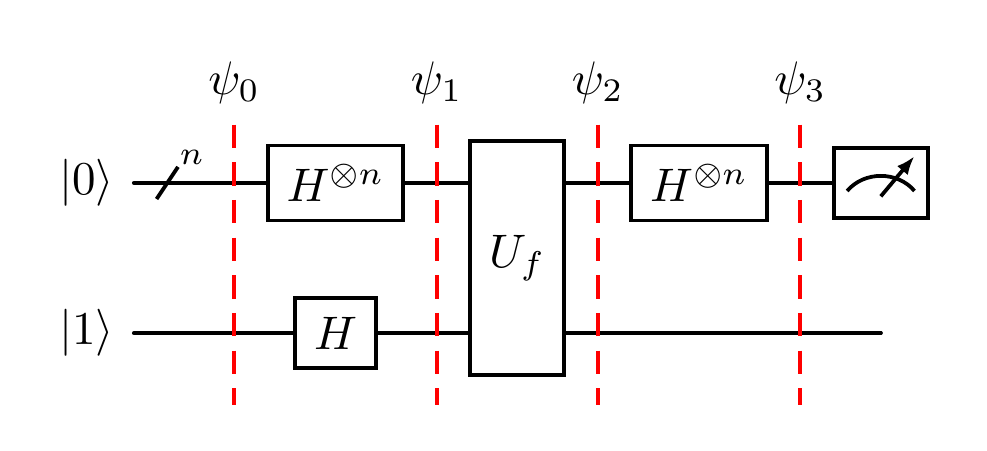
\begin{tikzpicture}
\node[scale=1.7]{
\begin{quantikz}
\lstick{$\ket{0}$} & \qwbundle{n} \slice{$\psi_0$} & \gate{H^{\otimes n}}\slice{$\psi_1$}  & \gate[2]{U_f}\slice{$\psi_2$}  & \gate{H^{\otimes n}}\slice{$\psi_3$} & \meter{} \\
\lstick{$\ket{1}$} & & \gate{H} & \qw & \qw & \qw
\end{quantikz}
};
\end{tikzpicture}
\end{align}

A zatem po kolei:
\begin{itemize}
    \item $\ket{\psi_0} = \ket{0}_n\ket{1}$
    \item Aplikujemy Hadamarda. Pamiętamy, że:
        \[ H\ket{0}_n = \frac{1}{\sqrt{2^n}}\sum_{x=0}^{2^n-1}\ket{x}, \qquad H\ket{1} = \ket{-} \]
        Zatem
        \[ \ket{\psi_1} = H\ket{\psi_0} = \frac{1}{\sqrt{2^n}}\sum_{x=0}^{2^n-1}\ket{x}\ket{-} \]
    \item Aplikujemy wyrocznię $U_f$. Wiemy, że działa ona tak:
        \[ U_f\ket{x}_n\ket{y} = \ket{x}_n\ket{y\otimes f(x)} \]
        Czyli:
        \[ U_f\ket{x}_n\ket{-} = U_f\ket{x}_n\left(\frac{\ket{0}-\ket{1}}{\sqrt2}\right)
        = \ket{x}_n\left(\frac{\ket{f(x)}-\ket{f(x)\oplus 1}}{\sqrt2}\right) \]
        Zauważmy, po ''zignorowaniu'' ostatniego kubitu jedynym widocznym wynikiem $f(x)$ w układzie jest zmieniona faza (+1 lub -1). \\    
        Niech $\ket{g}$ oznacza stan ostatniego bitu. Wtedy mamy:
        \[ \ket{\psi_2} = U_f\ket{\psi_1} = \frac{1}{\sqrt{2^n}}\sum_{x=0}^{2^n-1}(-1)^{f(x)}\ket{x}\ket{g} \]
    \item Ponownie Hadamard. Pamiętając, że $H\ket{k} = \frac{1}{\sqrt{2^n}}\sum_{i=0}^{2^n-1}(-1)^{k\cdot i}\ket{i}$ otrzymujemy:
        \[ \ket{\psi_3} = H\ket{\psi_2} = \frac{1}{2^n}\sum_{x=0}^{2^n-1}\sum_{y=0}^{2^n-1}(-1)^{f(x)+x\cdot y}\ket{y}\ket{g} \]
\end{itemize}
Dla uproszczenia analizy zapomnijmy o kubicie $\ket{g}$. Zauważmy, że dla konkretnego $y$:
\[\frac{1}{2^n}\sum_{x=0}^{2^n-1}(-1)^{f(x)+x\cdot y}
= \frac{1}{2^n}\sum_{x=0}^{2^n-1}(-1)^{x\cdot s+x\cdot y} 
= \frac{1}{2^n}\sum_{x=0}^{2^n-1}(-1)^{x\cdot(s\oplus y)} \] 
Łatwo zauważyć, że gdy $s=y$ to $s\oplus y = 0$ i wyrażenie jest równe 1. Jeśli natomiast $s\ne y$ to $s\oplus y$ będzie przyjmowało wartości 0 i 1 dla tej samej ilości wyrazów, więc wyrażenie się wyzeruje. \\ 
Czyli prawdopodobieństwo zmierzenia stanu $\ket{s}$ na pierwszych $n$ kubitach wynosi 1.
\end{proof}

% ------------------------------------------------------------------------------------------
\newpage
\section{Algorytm Grovera}
\begin{problem*}{}
    Dana czarna skrzynka w postaci funkcji $f: \{0,1\}^n \rightarrow \{0,1\}$. Funkcja ta zawsze przyjmuje wartość $0$, poza jednym nieznanym argumentem $\omega$, dla którego $f(\omega)=1$. \\
    Zadanie polega na znalezieniu wartości $\omega$.
\end{problem*}
W przypadku klasycznym widać, że potrzebne jest średnio $\frac{N}{2}$, a pesymistycznie $N-1$ ewaluacji funkcji $f$ do wyznaczenia $\omega$. \\
My dokonamy czegoś niesamowitego i wyznaczymy nieznaną wartość używając jedynie $\Os(\sqrt{N})$ ewaluacji $f$. \\
Użyjemy do tego dwóch operatorów:
\begin{itemize}
    \item $U_\omega := I - 2\ketbra{\omega}{\omega}$
    \item $U_s := 2\ketbra{s}{s} - I$
\end{itemize}
Oba są odbiciami Householdera. Oznacza to tyle, że jeśli rozważymy płaszczyznę rozpiętą przez wektory $\ket{\omega}$ i $\ket{\omega^\bot}$ to: 
\begin{itemize}
    \item $U_\omega$ odbija każdy wektor względem płaszczyzny $\ket{\omega^\bot}$ (prostopadłej do $\ket{\omega}$).
    \item $U_s$ odbija wektor względem $\ket{s}$
\end{itemize}
Załóżmy, że początkowo dany jest wektor $\ket{s}$, którego początkowy kąt z $\ket{\omega^\bot}$ wynosi $\theta$. Wtedy przekształcenie $U_s U_\omega$ graficznie wygląda następująco:

\begin{align}   
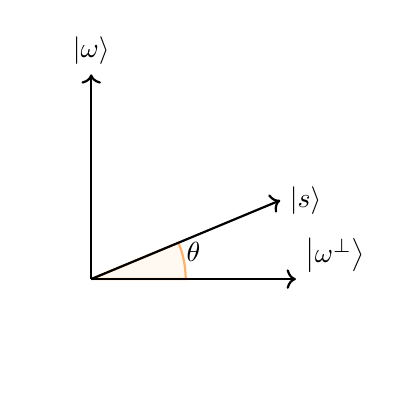
\begin{tikzpicture}[scale=0.2]{
    \filldraw[draw=orange!60, fill=orange!5, thick] (0,0) -- (6,0) arc (0:22.6198649481:6) -- (0,0) ;
    \draw[black, thick, ->] (0,0) -- (13,0);
    \draw[black, thick, ->] (0,0) -- (0,13);
    \draw[black, thick, ->] (0,0) -- (12,5);
    \filldraw[black] (-4,-6.3) node[anchor=west]{}; % fake
    \filldraw[black] (17,13) node[anchor=west]{}; % fake
    \filldraw[black] (12,5) node[anchor=west]{$\ket{s}$};
    \filldraw[black] (13,1.5) node[anchor=west]{$\ket{\omega^\bot}$};
    \filldraw[black] (0,13) node[anchor=south]{$\ket{\omega}$};
    \filldraw[black] (6.5,0.5) node[anchor=south]{$\theta$};
};
\end{tikzpicture} 
\qquad
\qquad
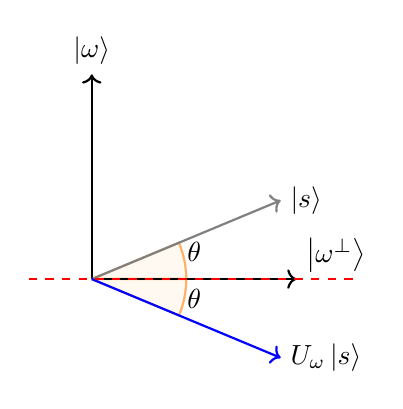
\begin{tikzpicture}[scale=0.2]{
    \filldraw[draw=orange!60, fill=orange!5, thick] (0,0) -- (6,0) arc (0:22.6198649481:6) -- (0,0) ;
    \filldraw[draw=orange!60, fill=orange!5, thick] (0,0) -- (6,0) arc (0:-22.6198649481:6) -- (0,0) ;
    \draw[black, thick, ->] (0,0) -- (13,0);
    \draw[black, thick, ->] (0,0) -- (0,13);
    \draw[gray, thick, ->] (0,0) -- (12,5);
    \draw[blue, thick, ->] (0,0) -- (12,-5);
    \draw[red, thick, dashed] (-4,0) to (17,0);
    \filldraw[black] (12,5) node[anchor=west]{$\ket{s}$};
    \filldraw[black] (13,1.5) node[anchor=west]{$\ket{\omega^\bot}$};
    \filldraw[black] (0,13) node[anchor=south]{$\ket{\omega}$};
    \filldraw[black] (6.5,0.5) node[anchor=south]{$\theta$};
    \filldraw[black] (6.5,-2.5) node[anchor=south]{$\theta$};
    \filldraw[black] (12,-5) node[anchor=west]{$U_\omega\ket{s}$};
};
\end{tikzpicture}
\qquad
\qquad
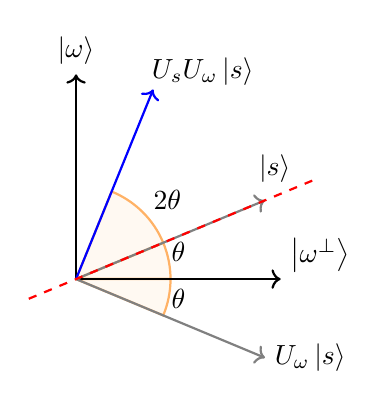
\begin{tikzpicture}[scale=0.2]{
    \filldraw[draw=orange!60, fill=orange!5, thick] (0,0) -- (6,0) arc (0:22.6198649481:6) -- (0,0) ;
    \filldraw[draw=orange!60, fill=orange!5, thick] (0,0) -- (6,0) arc (0:-22.6198649481:6) -- (0,0) ;
    \filldraw[draw=orange!60, fill=orange!5, thick] (0,0) -- (5.53846153846,2.30769230769) arc (22.6198649481:67.8595948442:6) -- (0,0) ;
    \draw[black, thick, ->] (0,0) -- (13,0);
    \draw[black, thick, ->] (0,0) -- (0,13);
    \draw[gray, thick, ->] (0,0) -- (12,5);
    \draw[gray, thick, ->] (0,0) -- (12,-5);
    \draw[blue, thick, ->] (0,0) -- (4.89940828403,12.0414201184);
    \draw[red, thick, dashed] (-3,-1.25) to (15,6.25);
    \filldraw[black] (11,7) node[anchor=west]{$\ket{s}$};
    \filldraw[black] (12,-5) node[anchor=west]{$U_\omega\ket{s}$};
    \filldraw[black] (13,1.5) node[anchor=west]{$\ket{\omega^\bot}$};
    \filldraw[black] (0,13) node[anchor=south]{$\ket{\omega}$};
    \filldraw[black] (6.5,0.5) node[anchor=south]{$\theta$};
    \filldraw[black] (6.5,-2.5) node[anchor=south]{$\theta$};
    \filldraw[black] (4.3,5) node[anchor=west]{$2\theta$};
    \filldraw[black] (4.2,11.7) node[anchor=south west]{$U_sU_\omega\ket{s}$};
};
\end{tikzpicture}
\end{align}

Przesunęliśmy się zatem w stronę $\ket{\omega}$ o kąt $2\theta$. Okazuje się, że każde kolejne zaaplikowanie $U_s U_\omega$ również przesuwa nas w stronę $\ket{\omega}$ o $2\theta$. Zatem możemy do skutku aplikować $U_s U_\omega$, a potem zmierzyć końcowy stan, który prawie na pewno będzie naszym szukanym $\ket{\omega}$. \\
Pozostaje jeszcze wybrać taki początkowy wektor $\ket{s}$, by $\theta>0$. Z braku lepszych opcji możemy ustalić $\ket{s} = H\ket{0}_n = \frac{1}{\sqrt{N}}\sum_{k=0}^{N-1} \ket{k}$. Sprawdźmy ile wtedy wynosi $\theta$:
\[ \cos \theta = \frac{\braket{s}{\omega^\bot}}{||s||\cdot ||\omega^\bot||} = \braket{s}{\omega^\bot} \]
Wiemy też, że
\[ \ket{s} = \frac{1}{\sqrt{N}}\sum_{k=0}^{N-1}\ket{k}
= \frac{1}{\sqrt{N}}\ket{\omega} + \frac{1}{\sqrt{N}}\sum_{k=0,k\ne\omega}^{N-1}\ket{k}
= \frac{1}{\sqrt{N}}\ket{\omega} + \frac{\sqrt{N-1}}{\sqrt{N}}\ket{\omega^\bot} \]
Zatem
\[ \braket{s}{\omega^\bot}
= \frac{1}{\sqrt{N}}\braket{\omega}{\omega^\bot}+\frac{\sqrt{N-1}}{\sqrt{N}}\braket{\omega^\bot}{\omega^\bot}
= \frac{\sqrt{N-1}}{\sqrt{N}} \]
\[ \Rightarrow \theta = \arccos \sqrt{\frac{N-1}{N} } \]
Z jedynki trygonometrycznej mamy
\[ \theta = \arcsin \frac{1}{\sqrt{N}} \]
Ale dla małych kątów $\arcsin x \approx x$, czyli $\theta \approx \frac{1}{\sqrt{N}}$. \\
Za każdym razem przesuwamy się o kąt $2\theta$, a chcemy aby kąt z początkowego $\approx 0$ stał się równy $\pi/2$. Łatwo zatem wyliczyć ilość potrzebnych zaaplikowań $U_sU_\omega$:
\[ \frac{\pi/2}{2\theta} \approx \frac{\pi/2\cdot \sqrt{N}}{2} = \boxed{\frac{\pi}{4}\sqrt{N}} = \Os(\sqrt N)\]   

Mamy już zatem gotowy algorytm (Grovera):
\begin{enumerate}
    \item Zainicjuj $\ket{s} := H\ket{0}_n$
    \item Zaaplikuj $\frac{\pi}{4}\sqrt{N}$ razy $U_s U_\omega$
    \item Zmierz końcowy rejestr
\end{enumerate}


\begin{definition*}{(BPP)}{}
    \textbf{Bounded-error polynomial time} (\textbf{BPP}) to klasa problemów decyzyjnych, które można rozwiązać w czasie wielomianowym, z prawdopodobieństwem pomyłki co najwyżej $\frac{1}{3}$ dla dowolnej z instancji.  
\end{definition*}

\begin{definition*}{(BQP)}{}
    \textbf{Bounded-error quantum polynomial time} (\textbf{BQP}) to klasa problemów decyzyjnych, które można rozwiązać w czasie wielomianowym \underline{na komputerze kwantowym}, z prawdopodobieństwem pomyłki co najwyżej $\frac{1}{3}$ dla dowolnej z instancji.  
\end{definition*}

Zachodzi następujące:
\[ P \sub BPP \sub BQP \sub PSPACE \] \\
Na dzień dzisiejszy dla żadnego z powyższych zawierań nie wiadomo czy są one ostre czy słabe.
\begin{definition*}{(Uniwersalny zbiór bramek)}{}
    Zbiór bramek $S$ nazywamy \textbf{uniwersalnym} jeśli dla każdej macierzy unitarnej $U\in\C^{N\times N}$ oraz $\varepsilon>0$ istnieje obwód $C$ złożony wyłącznie z bramek z $S$, nieużywający dodatkowych kubitów, taki, że dla każdego stanu $\ket{\psi}$ zachodzi
    \[ ||U\ket{\psi} - C\ket{\psi}|| \le \varepsilon \] 
\end{definition*}
Intuicyjnie zbiór bramek jest uniwersalny, gdy możemy zasymulować z dowolną prezycją dowolną operację $U$ możliwą na komputerze kwantowym.

% ------------------------------------------------------------------------------------------
\newpage
\section{Kubityzacja}
Macierze, których używamy w układach kwantowych muszą być unitarne. Co jednak w sytuacji, gdy chcemy wykonać operację niebędącą unitarną? Nie wszystko stracone - wystarczy zakodować wymarzoną przez nas macierz $A$ w większej macierzy $U_A$, poprzez dorzucenie dodatkowych kubitów (tzw. \textit{ancillas}):
\[ U_A = \mat{A,*}{*,*} \]  
gdzie wartości $*$ nas nie interesują, bo dotykają \textit{ancilla} kubitów. Nie interesują nas ich konkretne wartości, ale co ważne są one dobrane tak, że macierz całościowo jest unitarna. 
\begin{definition*}{(Block-encoding)}
    Mówimy, że $U_A$ to $(\alpha,a,\varepsilon)$-\textbf{block encoding} macierzy $A$, jeśli:
    \[ ||A-\alpha(_a\bra{0}\otimes \I_s)U_A(\ket{0}_a\otimes \I_s)|| \le \varepsilon \]
    gdzie $\alpha\in\R^+$, $\varepsilon\in\R^+$, $\ket{0}_a$ oznacza $\ket{0}^{\otimes a}$
\end{definition*}
Zapis $(_a\bra{0}\otimes \I_s)U_A(\ket{0}_a\otimes \I_s)$ oznacza tyle, że ''wycinamy'' z $U_A$ fragment reprezentujący macierz $A$. \\
Powyższa definicja jest dość ogólna. Zezwalamy by nasza macierz różniła się od wynikowej (w normie spektralnej) o co najwyżej $\varepsilon$. W definicji uwzględniamy również pewne przeskalowanie macierzy $A$ o współczynnik $\alpha$. Do samego zakodowania macierzy $U_A$ potrzebujemy też $a$ \textit{ancilla}-kubitów. 
\begin{example}
    Dla macierzy unitarnej $A$, samo $A$ jest jej $(1,0,0)$-block encoding'iem
\end{example}
\begin{lemma*}{}
    Niech $U_A$ i $U_B$ to odpowiednio $(\alpha, a, \varepsilon_A)$-BE dla macierzy $A$ i $(\beta, b, \varepsilon_B)$-BE dla macierzy $B$. \\
    Niech $U_{AB} := (I_b\otimes U_A)(I_a\otimes U_b)$. \\
    Wtedy $U_{AB}$ jest $(\alpha\beta, a+b, \alpha\varepsilon_B+\beta\varepsilon_A+\varepsilon_A\varepsilon_B)$-BE dla macierzy $AB$.
\end{lemma*}

\subsection{LCU}
\textbf{Linear Decomposition of Unitaries} (LCU) to metoda wyznaczania block-encoding'u dla zadanej macierzy $A$. \\
Sam algorytm jest dość nieskomplikowany. Najpierw, zapiszmy $A$ jako sumę macierzy unitarnych $U_k$:
\[ A = \sum_{k=0}^{N-1} \alpha_kU_k \]
gdzie $N=2^{n+a}$, $\alpha_i\in\R$. \\
Teraz zdefiniujmy operatory $PREP$ i $SEL$:
    \[ PREP\ket{0} = \sum_{k=0}^{N-1}\sqrt{\frac{|\alpha_k|}{\lambda}}|\ket{k} \]
    \[ SEL\ket{k}\ket{\psi} = \ket{k}U_k\ket{\psi} \] \\
gdzie wspólczynnik normalizacji $\lambda$ jest zdefiniowany jako $\lambda = \sum_{k=0}^{N-1} |\alpha_k|$. \\

Zdefiniujmy teraz $U_A$ jako
    \[U_A := PREP^\dagger \cdot SEL \cdot PREP \] \\
Okazuje się, że $U_A$ jest $(\lambda, a, 0)$-block encoding'iem $A$. Oznacza to, że możemy skonstruować taki układ:

\begin{align}
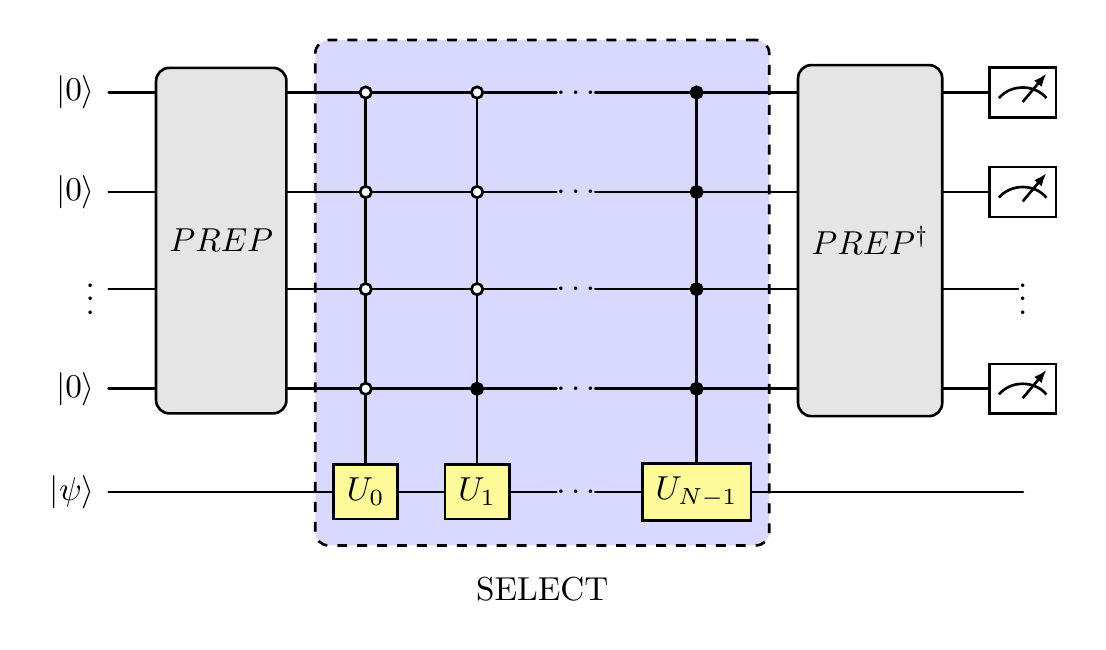
\begin{tikzpicture}
\node[scale=1.2]{
\begin{quantikz}
\lstick{$\ket{0}$} & \gate[style={fill=gray!20, rounded corners},4]{PREP} & \octrl{4}
\gategroup[5,steps=4,style={dashed,rounded corners,fill=blue!15,inner xsep=2pt},background,label style={label position=below,anchor=north,yshift=-0.4cm}]{{SELECT}}
    & \octrl{4}    & \ldots & \ctrl{4}       & \gate[style={fill=gray!20, , rounded corners},4]{PREP^\dagger}   & \meter{} \\
 \lstick{$\ket{0}$}     & \qw                                  & \ocontrol{} & \ocontrol{} & \ldots & \control{}     & \qw & \meter{} \\
 \lstick{$\vdots$}      & \qw                                  & \ocontrol{} & \ocontrol{} & \ldots & \control{}     & \qw & \vdots \\
 \lstick{$\ket{0}$}     & \qw                                  & \ocontrol{} & \control{} & \ldots & \control{}     & \qw & \meter{} \\
 \lstick{$\ket{\psi}$}  & \qw                                  & \gate[style={fill=yellow!40}]{U_0}  & \gate[style={fill=yellow!40}]{U_1}  & \ldots & \gate[style={fill=yellow!40}]{U_{N-1}} & \qw & \qw 
\end{quantikz}
};
\end{tikzpicture}
\end{align}
Jeśli teraz go uruchomimy, oraz na wszystkich (górnych) $a$ miernikach zmierzymy $\ket{0}$, to końcowy stan na ostatniej (dolnej) linii będzie równy $\frac{A}{\lambda}\ket{\psi}$.

\begin{proof}
    Przeanalizujmy dokładnie co się dzieje w tym układzie

\begin{align}
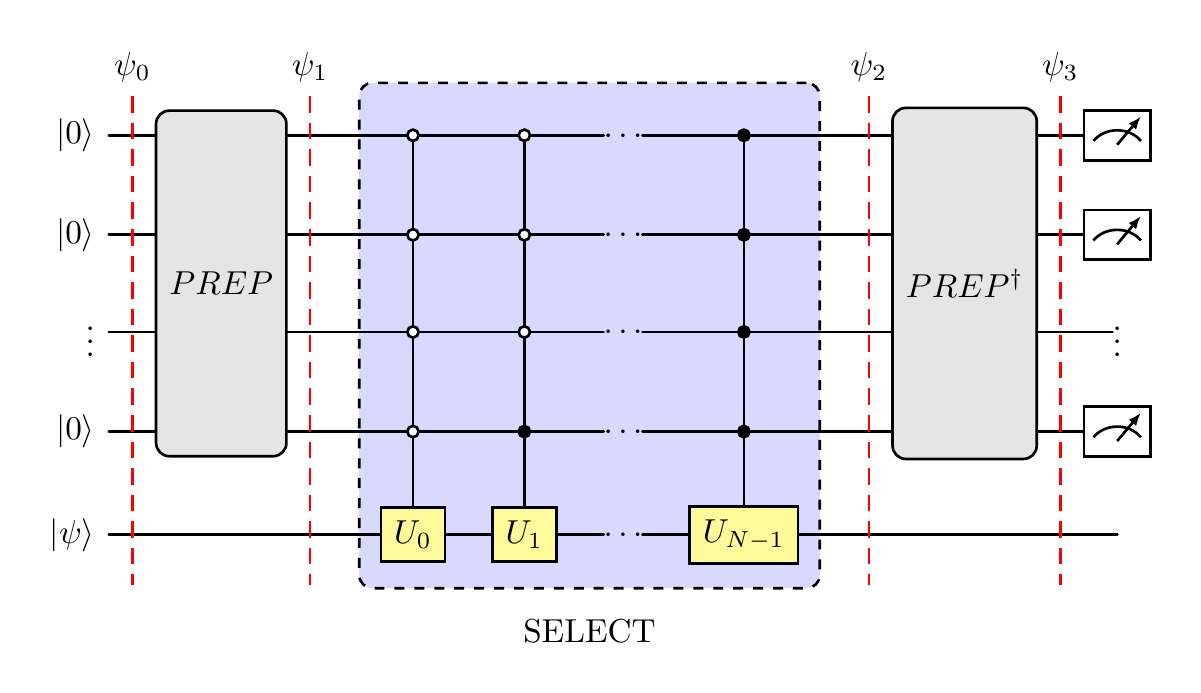
\begin{tikzpicture}
\node[scale=1.2]{
\begin{quantikz}
\lstick{$\ket{0}$}\slice{$\psi_0$} & \gate[style={fill=gray!20, rounded corners},4]{PREP}\slice{$\psi_1$} & \qw & \octrl{4}
\gategroup[5,steps=4,style={dashed,rounded corners,fill=blue!15,inner xsep=3pt},background,label style={label position=below,anchor=north,yshift=-0.4cm}]{{SELECT}}
    & \octrl{4}    & \ldots & \ctrl{4}      & \qw\slice{$\psi_2$} & \gate[style={fill=gray!20, , rounded corners},4]{PREP^\dagger}\slice{$\psi_3$}   & \meter{} \\
\lstick{$\ket{0}$}     & & \qw                                  & \ocontrol{} & \ocontrol{} & \ldots & \control{}     & & \qw & \meter{} \\
\lstick{$\vdots$}      & & \qw                                  & \ocontrol{} & \ocontrol{} & \ldots & \control{}     & & \qw & \vdots \\
\lstick{$\ket{0}$}     & & \qw                                  & \ocontrol{} & \control{} & \ldots & \control{}     & & \qw & \meter{} \\
\lstick{$\ket{\psi}$}  & & \qw                                  & \gate[style={fill=yellow!40}]{U_0}  & \gate[style={fill=yellow!40}]{U_1}  & \ldots & \gate[style={fill=yellow!40}]{U_{N-1}} & & \qw & \qw 
\end{quantikz}
};
\end{tikzpicture}
\end{align}

\begin{itemize}
    \item $\ket{\psi_0} = \ket{0}_a\ket{\psi}$
    \item Aplikujemy $PREP$:
        \[ \ket{\psi_1} = PREP\ket{0}\ket{\psi_0} = \sum_{k=0}^{N-1}\sqrt{\frac{|\alpha_k|}{\lambda}}\ket{k}\ket{\psi}  \] \\
    \item Aplikujemy $SEL$:
        \[ \ket{\psi_2} = SEL\ket{\psi_1} = \sum_{k=0}^{N-1}\sqrt{\frac{|\alpha_k|}{\lambda}}SEL\ket{k}\ket{\psi}
            = \sum_{k=0}^{N-1}\sqrt{\frac{|\alpha_k|}{\lambda}}\ket{k}U_k\ket{\psi}
        \] \\
    \item Aby poznać $\ket{\psi_3}$ przyjrzyjmy się jak działa $PREP^\dagger$:
        \[ \bra{0}PREP^\dagger = (PREP\ket{0})^\dagger = \left(\sum_{k=0}^{N-1}\sqrt{\frac{|\alpha_k|}{\lambda}}\ket{k}\right)^\dagger
        = \sum_{k=0}^{N-1}\sqrt{\frac{|\alpha_k|}{\lambda}}\bra{k} \] \\
        Uzbrojeni w tą wiedzę dostajemy, że:
        \[ \ket{\psi_3} = \bra{0}PREP^\dagger \cdot \ket{\psi_2} = \left(\sum_{k=0}^{N-1}\sqrt{\frac{|\alpha_k|}{\lambda}}\bra{k}\right) \cdot \left(\sum_{k=0}^{N-1}\sqrt{\frac{|\alpha_k|}{\lambda}}\ket{k}U_k\ket{\psi}\right) \] \\
        Pogrupujmy pary wartości z obu sum względem tego czy są te same:
        \[  = \left(\sum_{i}\frac{|\alpha_i|}{\lambda}\braket{i}{i}U_i\ket{\psi}\right)
            + \left(\sum_{i\ne j}\frac{\sqrt{|\alpha_i|\cdot |\alpha_j|}}{\lambda}\braket{i}{j}U_j\ket{\psi}\right)
        \] \\
        Zauważmy, że skoro $\ket{i} \bot \ket{j}$ to $\braket{i}{i}=1$ oraz $\braket{i}{j}=0$ dla $i\ne j$. Kasuje się prawy nawias i otrzymujemy:
        \[ = \sum_{i=0}^{N-1} \frac{|\alpha_i|}{\lambda}U_i\ket{\psi}
           = \frac{1}{\lambda} \sum_{i=0}^{N-1} \alpha_iU_i\ket{\psi}
           = \frac{A}{\lambda}\ket{\psi}
        \] \\
\end{itemize}
\end{proof}

% ------------------------------------------------------------------------------------------
\newpage
\section{QFT}
\textbf{Kwantowa transformata Fouriera} (ang. Quantum Fourier Transform) to przekształcenie analogicze do Dyskretnej Transformaty Fouriera (DFT), tylko w przypadku kwantowym. Przypomnijmy najpierw definicję DFT:
\begin{definition*}{(DFT)}
    \textbf{Dyskretną transformatą Fouriera} nazywamy funkcję 
    \[ DFT:(x_0,\dots,x_{N-1}) \mapsto (y_0,\dots,y_{N-1})\]
    gdzie
    \[ y_k = \frac{1}{\sqrt{N}}\sum_{j=0}^{N-1}x_j\omega^{-jk} \] \\
    \[ \omega = \sqrt[N]{1}=e^{2\pi i/N} \]
\end{definition*}

Podobnie możemy sformułować QFT.

\begin{definition*}{(QFT)}
    Niech $\ket{x} = \sum_{j=0}^{N-1}x_j\ket{j}$. \\
    \textbf{Kwantową transformatą Fouriera} nazywamy funkcję
    \[ QFT:\ket{x} \mapsto \frac{1}{\sqrt{N}}\sum_{k=0}^{N-1} \omega^{xk}\ket{k} \]
\end{definition*}

Można jednak patrzeć na to w inny sposób. Niech macierz Fouriera $F_N$ będzie określona następująco:
\[
F_N = \frac{1}{\sqrt{N}}
\mat{1,1,1,\dots,1}{1,\omega,\omega^2,\dots,\omega^{N-1}}{\vdots,\vdots, \vdots,\ddots,\vdots}{1,\omega^{N-1},\omega^{2(N-1)},\dots,\omega^{(N-1)(N-1)}}
\]
Wtedy, przyjmując $X=(x_0,\dots,x_{N-1})$, $Y=(y_0,\dots,y_{N-1})$ mamy, że:
\[ DFT(X) = X\cdot F_N = Y \] \\
Łatwo można sprawdzić, że macierz $F_N$ jest unitarna. Zatem jest ona poprawną bramką kwantową. Oznacza to ni mniej ni więcej tyle, że QFT można traktować właśnie jako zaaplikowanie bramki $F_N$:
\[ QFT\ket{x} \iff* F_N\ket{x} \]  \\
Teraz postaramy się skonstruować obwód dla $F_N$. Niech zapis $0.k_1k_2\dots k_{n}$ oznacza liczbę zapisaną binarnie, przy pomocy bitów $k_1,\dots,k_n$. Wtedy zachodzi:
\[ QFT\ket{k} = QFT\ket{k_1}\dots\ket{k_{n}} \]
\[ = \frac{1}{\sqrt{N}}\left(\ket{0}+e^{2\pi i\cdot 0.k_n}\ket{1}\right)\oplus \left(\ket{0}+e^{2\pi i\cdot 0.k_{n-1}k_n}\ket{1}\right)\oplus \dots \oplus \left(\ket{0}+e^{2\pi i\cdot 0.k_1\dots k_n}\ket{1}\right) \]

% \begin{proof}
%     TODO
% \end{proof}
Reprezentacja ta jest o tyle pomocna, że przedstawiamy wyjście jako produkt tensorowy pojedynczych kubitów. Będą nam teraz potrzebne jedynie dwie bramki: $H$ i $R_k$:
\[ H = \frac{1}{\sqrt2} \mat{1,1}{1,-1} \] 
\[ R_k = \mat{1,0}{1,e^{2\pi i / 2^k}} \]
Wtedy nasz układ prezentuje się następująco (na wyjściach dla czytelności pominięty współczynnik $\frac{1}{\sqrt{2}}$):

\begin{align}
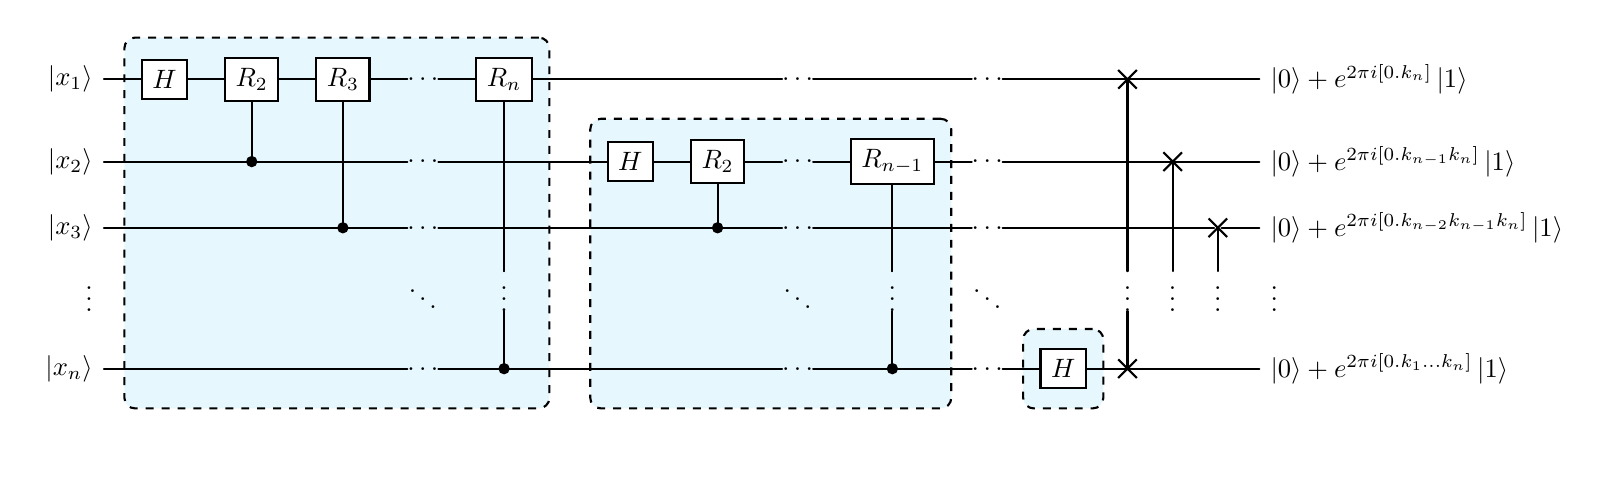
\begin{tikzpicture}
\node[scale=0.96]{
\begin{quantikz}
\lstick{$\ket{x_1}$} & \gate{H}
\gategroup[5,steps=5,style={dashed,rounded corners,fill=cyan!10,inner xsep=3pt},background,label style={label position=below,anchor=north,yshift=-0.4cm}]{{}}
& \gate{R_2} & \gate{R_3} & \ldots & \gate{R_n} & & & & \ldots & & \ldots & & \swap{2} & & & \rstick{$\ket{0} + e^{2\pi i[0.k_n]}\ket{1}$} \\
\lstick{$\ket{x_2}$} & & \control{1} \wire[u]{q} &  \wire[u]{q}\wire[d]{q} & \ldots & \wire[u]{q}\wire[d]{q} & & \gate{H}
\gategroup[4,steps=4,style={dashed,rounded corners,fill=cyan!10,inner xsep=3pt},background,label style={label position=below,anchor=north,yshift=-0.4cm}]{{}}
& \gate{R_2} & \ldots & \gate{R_{n-1}} & \ldots & & & \swap{1} & & \rstick{$\ket{0} + e^{2\pi i[0.k_{n-1}k_n]}\ket{1}$}  \\
\lstick{$\ket{x_3}$} & & & \control{1} & \ldots & \wire[u]{q}\wire[d]{q} & & & \control{1}\wire[u]{q} & \ldots & \wire[u]{q}\wire[d]{q} & \ldots & & & & \swap{0} & \rstick{$\ket{0} + e^{2\pi i[0.k_{n-2}k_{n-1}k_n]}\ket{1}$} \\
\lstick{\vdots} &\setwiretype{n} & & & \ddots & \push{\vdots}\wire[u]{q}\wire[d]{q} & & & & \ddots & \push{\vdots}\wire[u]{q}\wire[d]{q} & \ddots & & \push{\vdots}\wire[u]{q}\wire[d]{q} & \push{\vdots}\wire[u]{q} & \push{\vdots}\wire[u]{q}  & \rstick{\vdots} \\
\lstick{$\ket{x_n}$} & & & & \ldots & \control{1}\wire[u]{q} & & & & \ldots & \control{1} & \ldots & \gate{H}
\gategroup[1,steps=1,style={dashed,rounded corners,fill=cyan!10,inner xsep=3pt},background,label style={label position=below,anchor=north,yshift=-0.4cm}]{{}}
& \targX{} & & & \rstick{$\ket{0} + e^{2\pi i[0.k_1\ldots k_n]}\ket{1}$} 
    \end{quantikz}
};
\end{tikzpicture}
\end{align}

\begin{proof}
    Zauważmy, że przy naszych oznaczeniach $H=\frac{1}{\sqrt{2}} R_1$. Zatem, jeśli prześledzimy pojedynczy kabel dojdziemy do wniosku, że domnażając wszystko do siebie otrzymamy \textit{prawie} to czego potrzebujemy. Prawie, bo wszystko będzie w odwrotnej kolejności. Dlatego potrzebujemy jeszcze na końcu zamienić bity miejscami bramkami $SWAP$.
\end{proof}
Nasz układ posiada $n$ bramek $H$, $(n-1)+\dots+2+1=\frac{n(n-1)}{2}$ $R_k$ oraz $\floor{\frac{n}{2}} SWAP$. Sumarycznie mamy zatem $\Os(n^2)$ bramek. \\
Jest to znakomity wynik, gdyż w klasyczne DFT wymaga $\Os(n2^n)$ operacji.  

\subsection{Quantum Phase Estimation}
\begin{problem*}{}
    Dany jest unitarny operator $U$ oraz stan własny $\ket{\psi}$. A zatem możemy go zapisać jako:
    \[ U\ket{\psi} = e^{2\pi i\phi}\ket{\psi} \]
    Zadaniem jest wyznaczenie wartości $\phi$.
\end{problem*}
Zauważmy, że skoro $\phi\in[0,1]$ to możemy traktować $\ket{\phi}$ jako stan odpowiadający zapisowi binarnemu $\phi$. Zobaczmy co się stanie po zaaplikowaniu QFT na nim:
\[ QFT\ket{\phi} = \frac{1}{\sqrt{2^n}}\sum_{k=0}^{2^n-1} e^{2\pi i\phi k}\ket{k} \]
Wygląda podobnie do naszego $U$, ale nie do końca. Zapamiętajmy jednak, że jak zobaczymy wyrażenie po prawej, to operacją $QFT^\dagger$ możemy odzyskać $\phi$. \\
Mamy zatem superpozycję stanów $U^k\ket{\phi}$:
\[ U^k\ket{\psi} = e^{2\pi i\phi k}\ket{\psi} \]
Zauważmy, że gdybyśmy znaleźli operator $SEL'$ zachowujący się następująco:
\[ SEL'\ket{k}\ket{\psi} = \ket{k}U^k\ket{\psi} \]
To umielibyśmy skonstruować cały układ:
\[
    \ket{0}_n\ket{\psi}
    \xmapsto{H^{\otimes n}\otimes I}
    \frac{1}{\sqrt{2^n}}\sum_{k=0}\ket{k}\ket{\psi}
    \xmapsto{SEL'}
    \frac{1}{\sqrt{2^n}}\sum_{k=0}\ket{k}U^k\ket{\psi}
    = \frac{1}{\sqrt{2^n}}\left(\sum_{k=0}e^{2\pi i \phi k}\ket{k}\right)\ket{\psi}
    \xmapsto{QFT^\dagger\otimes I}
    \ket{\phi}\ket{\psi}
\]
Okazuje się, że $SEL'$ nie jest tak trudny do skonstruowania: \\
\begin{align}
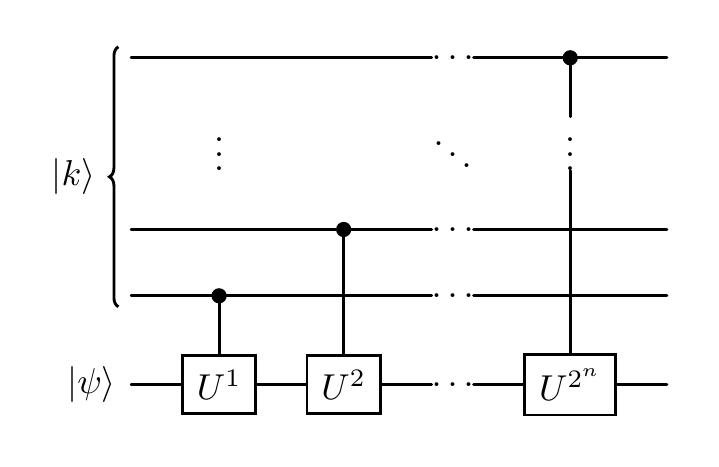
\begin{tikzpicture}
\node[scale=1.3]{
\begin{quantikz}
\lstick[4]{$\ket{k}$} &            &            & \ldots & \control{}                          &  \\    
\setwiretype{n}       & \vdots     &            & \ddots & \push{\vdots}\wire[u]{q}\wire[d]{q} &  \\ 
                      &            &  \ctrl{2}  & \ldots & \wire[d]{q}                         &  \\    
                      & \ctrl{1}   &            & \ldots & \wire[d]{q}                         &  \\    
\lstick{$\ket{\psi}$} & \gate{U^1} & \gate{U^2} & \ldots & \gate{U^{2^n}}                      &   
\end{quantikz}
};
\end{tikzpicture}
\end{align}
Jeśli przyjrzymy się ostatniemu kablowi i temu co do niego domnażamy to dojdziemy do wniosku, że faktycznie układ spełnia swoje zadanie. Stan $\ket{k}$ odpowiada zapisowi binarnemu $k$, a zatem jeśli odpowiedni bit $i$ będzie zapalony w $k$ to domnożymy do wyniku odpowiednią potęgę $U^{2^i}$. \\
Mamy już wszystko. Możemy zatem podziwiać końcowy układ w pełnej okazałości: \\
\begin{align}
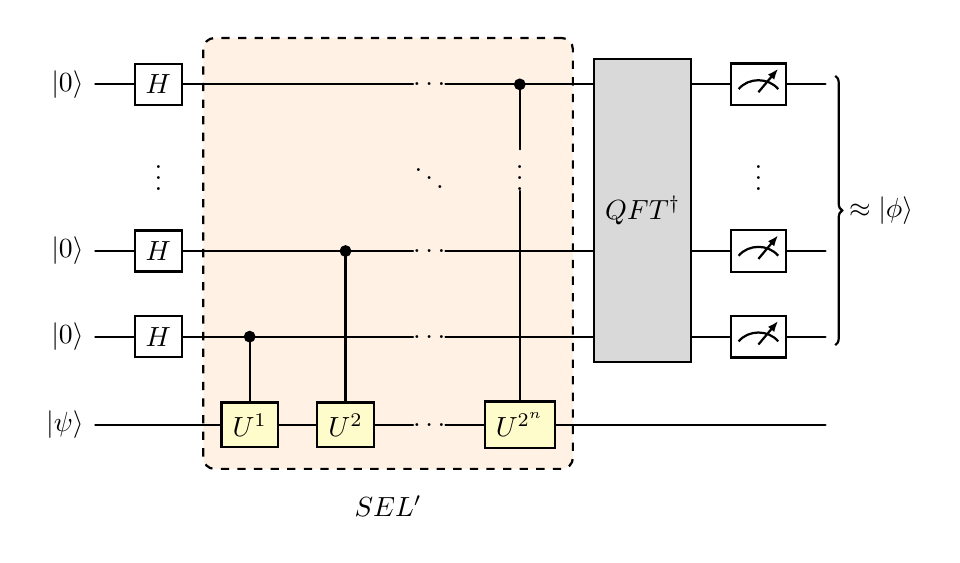
\begin{tikzpicture}
\node[scale=1.0]{
\begin{quantikz}
\lstick{$\ket{0}$}     & \gate{H} & \gategroup[5,steps=4,style={dashed,rounded corners,fill=orange!10,inner xsep=3pt},background,label style={label position=below,anchor=north,yshift=-0.4cm}]{{$SEL'$}}           &            & \ldots & \control{}                          & \gate[style={fill=gray!30},4]{QFT^\dagger} & \meter{} & \rstick[4]{$\approx\ket{\phi}$}\\    
\setwiretype{n}        & \vdots   &            &            & \ddots & \push{\vdots}\wire[u]{q}\wire[d]{q} &                       & \vdots   & \\ 
\lstick{$\ket{0}$}     & \gate{H} &            & \ctrl{2}   & \ldots & \wire[d]{q}                         &                       & \meter{} & \\    
\lstick{$\ket{0}$}     & \gate{H} & \ctrl{1}   &            & \ldots & \wire[d]{q}                         &                       & \meter{} & \\    
\lstick{$\ket{\psi}$}  &          & \gate[style={fill=yellow!20}]{U^1} & \gate[style={fill=yellow!20}]{U^2} & \ldots & \gate[style={fill=yellow!20}]{U^{2^n}}                      &                       &          & 
\end{quantikz}
};
\end{tikzpicture}
\end{align}

\subsection{Phase kickback}
\begin{definition*}{}{}
    \textbf{Phase kickback} to sytuacja, w której kubity kontrolowane mają wpływ na kubity je kontrolujące.
\end{definition*}
\begin{example}
Rozważmy dowolną bramkę CU (controlled unitary): 
\begin{align}
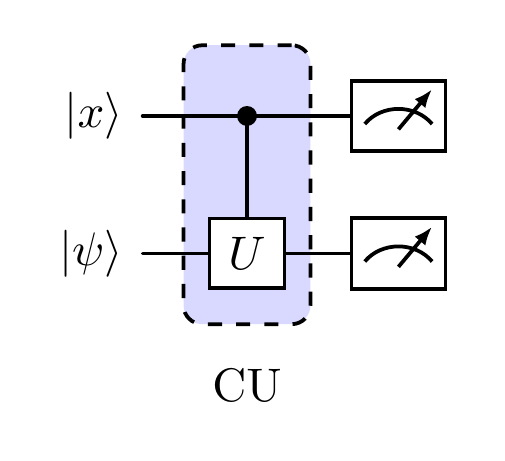
\begin{tikzpicture}
\node[scale=1.7]{
\begin{quantikz}
\lstick{$\ket{x}$} & \ctrl{1}\gategroup[2,steps=1,style={dashed,rounded corners,fill=blue!15,inner xsep=2pt},background,label style={label position=below,anchor=north,yshift=-0.4cm}]{{CU}} & \meter{} \\
\lstick{$\ket{\psi}$} & \gate{U}  & \meter{}
\end{quantikz}
};
\end{tikzpicture}
\end{align}
Jest kontrolowana, czyli będzie się zachowywać następująco:
\[ CU\ket{0}\ket{\psi} = \ket{0}\ket{\psi} \]
\[ CU\ket{1}\ket{\psi} = \ket{1}U\ket{\psi} \]
Niech dodatkowo $\ket{\psi}$ będzie stanem własnym (eigenstate) U, czyli:
\[ U\ket{\psi} = e^{2\pi i \phi}\ket{\psi} \]
dla pewnego $\phi$. Ale uwaga, bo teraz jeśli popatrzymy dowolny stan $\ket{x} = \alpha\ket{0} + \beta\ket{1}$ to otrzymujemy:
\[ CU\ket{x}\ket{\psi} \enspace = \enspace CU\left[(\alpha\ket{0} + \beta\ket{1})\otimes\ket{\psi}\right] \enspace = \enspace \alpha CU (\ket{0}\ket{\psi}) + \beta CU (\ket{1}\ket{\psi}) \]
\[ = \enspace \alpha\ket{0}\ket{\psi} + \beta e^{2\pi i \phi}\ket{1}\ket{\psi} \enspace = \enspace \left(\alpha\ket{0} + \beta e^{2\pi i \phi}\ket{1}\right)\ket{\psi} \] \\

Jeśli przypatrzymy się wejściu i wyjściu dojdziemy do ciekawego wniosku - ''wynikowy'' stan $\ket{\psi}$ ma wpływ na wartość pierwszego kubitu. \\
Właśnie tego typu efekt rozumiemy przez \textit{phase kickback}.
\end{example}

\subsection{Hamiltonian simulations}
Jak wszyscy dobrze pamiętamy równanie Schrödingera wygląda z grubsza tak:
\[ i\hbar \frac{d}{dt}\ket{\psi(t)} = H\ket{\psi(t)}\]
gdzie $\ket{\phi_t} = \ket{\phi(t)}$. Niech $\ket{\psi_0}$ oznacza stan początkowy. \\
Zakładając, że $H(t)=H$ to rozwiązanie przedstawia się następująco:
\[ \ket{\psi_t} = e^{-i t H / \hbar} \ket{\psi_0} = U(t)\ket{\psi_0} \]
Czyli:
\[ U(t) = e^{-i H t} \]
Chcielibyśmy wyznaczyć $U(t)$. Jednak problemem jest rozmiar $H$ oraz fakt, że chcemy policzyć $e^{H\cdot\dots}$. Otóż $H$ ma rozmiary $2^n\times 2^n$ co już dla dziesiątek kubitów daje olbrzymie macierze, z których jeszcze trzeba policzyć eksponens. \\
Z tego powodu wystarczy nam wyznaczenie $U'(t) \approx U(t)$. Aby pokonać problemy obliczeniowe skorzystamy z faktu, że:
\[ e^{-i H t } = \lim_{L\rightarrow \infty} \left( e^{-i \frac{t}{L} H_1 }e^{-i \frac{t}{L} H_2 } \right)^L \] \\
 
gdzie $H = H_1 + H_2$. Będziemy próbowali tak ustalić $H_1,H_2$, by łatwo dało się z nich policzyć $\exp$. \\
Na nasze potrzeby $L<\infty$, więc będą występować błędy. Niech $\Delta t = \frac{t}{L}$. Wtedy zachodzą następujące zależności:
\[ ||e^{-i\Delta t H} - e^{-i\Delta t H_1}e^{-i\Delta t H_2} || = \Os(\Delta t^2) \] 
\[ ||e^{-i t H} - e^{-i t H_1}e^{-i t H_2} || = \Os\left(\frac{t^2}{L}\right) \] 

% TODO:  notatki z Teamsów ... 
% ------------------------------------------------------------------------------------------
\newpage
\section{Algorytm Shor'a}
\subsection{Problem Simona}
\begin{problem*}{}
    Dana jest czarna skrzynka w postaci funkcji $f: \{0,1\}^n \rightarrow \{0,1\}^m,\; m\ge n$. Mamy gwarancję, że istnieje wartość $s$, dla której:
    \[ f(x)=f(x') \iff* x=x'\oplus s \]
    Zadaniem jest wyznaczenie wartości $s$. \\
    Chcemy również wykonać możliwie mało ewaluacji funkcji $f$.
\end{problem*}

Klasyczne podejście polegałoby na ciągłym ewaluowaniu $f$ i obserwowaniu, czy nie otrzymaliśmy uzyskanej już wcześniej wartości. Jednak mamy aż $2^n$ argumentów do sprawdzenia. Nawet uwzględniając paradoks urodzin, rozwiązanie będzie wymagało średnio $\Os{\sqrt{2^n}}$ ewaluacji funkcji $f$. \\

My jednak zaprezentujemy algorytm kwantowy, który pozwoli wyznaczyć $s$ z dużym prawdopodobieństwem, przy użyciu $\Os(n)$ zapytań o funkcję $f$. Głównym elementem będzie następujący obwód: 

\begin{align}
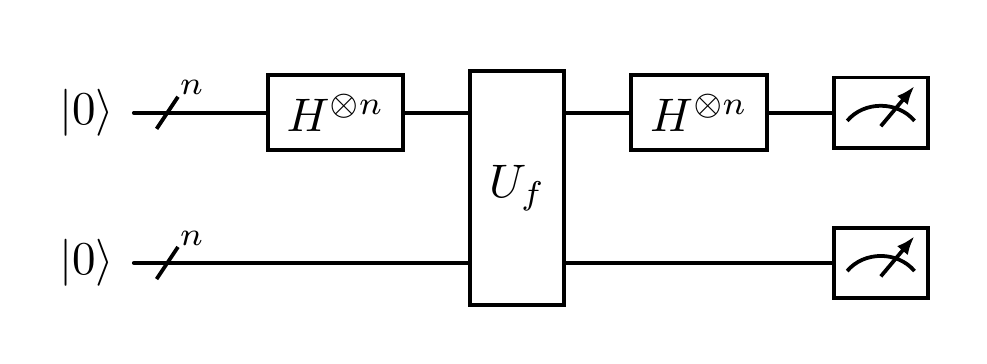
\begin{tikzpicture}
\node[scale=1.7]{
\begin{quantikz}
\lstick{$\ket{0}$} & \qwbundle{n} & \gate{H^{\otimes n}}  & \gate[2]{U_f}  & \gate{H^{\otimes n}} & \meter{} \\
\lstick{$\ket{0}$} & \qwbundle{n} &                       &                &                      & \meter{}
\end{quantikz}
};
\end{tikzpicture}
\end{align}

Sam algorytm przedstawia się następująco:
\begin{enumerate}
    \item Uruchom powyższy układ odpowiednią ilość razy, generując zbiór liniowo niezależnych wektorów bitowych $y_1,\dots,y_{n-1}$, \textbf{prostopadłych do $s$}.
    \item Każde wygenerowane $y_k$ spełnia $y_k\cdot s = 0$. Z tego układu równań wyznaczamy wartość $s$.
\end{enumerate}
I to wszystko. \\
Pozostaje tylko kwestia, dlaczego to w ogóle działa. W tym celu pokażemy dwie rzeczy:
\begin{enumerate}[label = (\roman*)]
    \item Każdy wektor wygenerowany przez układ jest prostopadły do $s$.
    \item Szansa, że wszystkie $y_1,\dots,y_{n-1}$ są liniowo niezależne jest niemała.
\end{enumerate}
\begin{proof}\textbf{(i)} \\

W tym celu musimy przeanalizować działanie układu krok po kroku:
\begin{align}
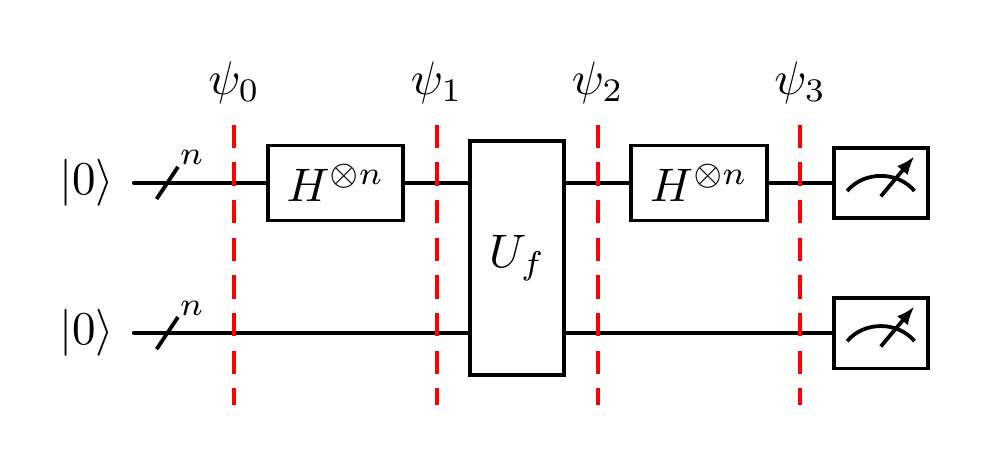
\begin{tikzpicture}
\node[scale=1.7]{
\begin{quantikz}
\lstick{$\ket{0}$} & \qwbundle{n}\slice{$\psi_0$} & \gate{H^{\otimes n}}\slice{$\psi_1$}  & \gate[2]{U_f}\slice{$\psi_2$}  & \gate{H^{\otimes n}}\slice{$\psi_3$} & \meter{} \\
\lstick{$\ket{0}$} & \qwbundle{n} &                       &                &                      & \meter{}
\end{quantikz}
};
\end{tikzpicture}
\end{align}
    \begin{itemize}
        \item $\ket{\psi_0} = \ket{0}_n\ket{0}_n$
        \item Bramka Hadamarda działa tak:
            \[ H\ket{0}_n = \frac{1}{\sqrt{2^n}}\sum_{k=0}^{2^n-1}\ket{k} \]
        A więc:
            \[ \ket{\psi_1} = (H\otimes I_n)\ket{\psi_0} = \frac{1}{\sqrt{2^n}}\sum_{k=0}^{2^n-1}\ket{k}\ket{0}_n \]
        \item Wyrocznia $U_f$ działa tak:
        \[ U_f\ket{x}\ket{y} = \ket{x}\ket{y\oplus{f(x)}} \]
        Zatem:
        \[ \ket{\psi_2} = U_f\ket{\psi_1} = \frac{1}{\sqrt{2^n}}\sum_{k=0}^{2^n-1}\ket{k}\ket{f(k)}  \]
        \item Hadamard działa też tak:
            \[ H\ket{k} = \frac{1}{\sqrt{2^n}} \sum_{j=0}^{2^n-1} (-1)^{k\cdot j}\ket{j} \]
        To daje nam
        \[ \ket{\psi_3} = (H\otimes I_n)\ket{\psi_2} = \frac{1}{\sqrt{2^n}}\sum_{k=0}^{2^n-1}\left[\frac{1}{\sqrt{2^n}} \sum_{j=0}^{2^n-1}(-1)^{k\cdot j}\ket{j}\right]\ket{f(k)} \]
        \[ = \sum_{j=0}^{2^n-1}\ket{j}\left[\frac{1}{2^n}\sum_{k=0}^{2^n-1}(-1)^{j\cdot k}\ket{f(k)}\right] \]
        A zatem prawdopodobieństwo zmierzenia danego stanu $\ket{j}$ jest równe:
        \[ \left\|\frac{1}{2^n}\sum_{k=0}^{2^n-1}(-1)^{j\cdot k}\ket{f(k)} \right\|^2 \]
    \end{itemize}
    \begin{enumerate}[label=\arabic*)]
        \item $s = 0$: \\
        Wtedy mamy, że $f$ jest bijekcją. Z tego mamy, że:
        \[ \left\|\frac{1}{2^n}\sum_{k=0}^{2^n-1}(-1)^{j\cdot k}\ket{f(k)} \right\|^2 = \frac{1}{4^n}\sum_{k=0}^{2^n-1}\norm{(-1)^{j\cdot k}\ket{f(k)}}^2 = \frac{1}{4^n}\cdot 2^n = \frac{1}{2^n} \]
        \item $s \ne 0$: \\
        Wynika z tego, że $f(x_1)=f(x_2)=z$ dla pewnych $x_1,x_2$ oraz $z\in range(f)$. Czyli:
        \[ \norm{\frac{1}{2^n}\sum_{k=0}^{2^n-1}(-1)^{j\cdot k}\ket{f(k)} }^2 = \norm{\frac{1}{2^n}\sum_{z\in range(f)} \Bigl( (-1)^{j\cdot x_1}+(-1)^{j\cdot x_2} \Bigr)\ket{z}}^2 \]
        Korzystamy z faktu, że $x_2=x_1\oplus s$:
        \[ = \norm{\frac{1}{2^n}\sum_{z\in range(f)} \Bigl( (-1)^{j\cdot x_1}+(-1)^{j\cdot (x_1\oplus s)} \Bigr)\ket{z}}^2  \]
        \[ = \norm{\frac{1}{2^n}\sum_{z\in range(f)} \Bigl( (-1)^{j\cdot x_1}+(-1)^{j\cdot x_1 \oplus j\cdot s} \Bigr)\ket{z}}^2  \]
        \[ = \norm{\frac{1}{2^n}\sum_{z\in range(f)} (-1)^{j\cdot x_1}\Bigl(1 + (-1)^{j\cdot s} \Bigr)\ket{z}}^2  \]
        W tej postaci jest to łatwe to przeanalizowania:
        \begin{itemize}
            \item Jeśli $j\cdot s = 1$, to wyrażenie ewaluuje się do $0$.
            \item Jeśli $j\cdot s = 0$, to wyrażenie (postępując w analogiczny sposób jak w $1)$, pamiętając, że $|range(f)|=2^{n-1}$) jest równe $\frac{1}{2^{n-1}}$.
        \end{itemize} 
    \end{enumerate}
    Czyli możemy zmierzyć tylko takie $\ket{j}$, dla których zachodzi $j\cdot s = 0$.
\end{proof}
\begin{proof}\textbf{(ii)} \\
    Dane są wektory $y_1,\dots,y_{n-1}$. Jakie jest prawdopodobieństwo, że wszystkie są liniowo niezależne? \\
    Wektorów prostopadłych do $s$ jest $2^{n-1}$. Wcześniej wyliczyliśmy też, że każdy z nich ma tą samą szansę bycia wylosowanym. \\
    Zapytajmy się zatem dla każdego wektora $y_k$ jaka jest szansa, że jest on liniowo niezależny z każdym z $y_1,\dots,y_{k-1}$. \\

    Dla $y_1$ jedyna sytuacja, że wektor będzie liniowo zależny to gdy wylosuje się $000\dots0$. Szansa na to wynosi $\frac{1}{2^{n-1}}$, czyli szansa że jest lin. niez. wynosi $1-\frac{1}{2^{n-1}}$
    
    Dla $y_2$ zła sytuacja wystąpi wtedy, gdy wylosuje się $0$ lub $y_1$. Czyli szansa że $y_2$ będzie liniowo niezależny wynosi $1-\frac{1}{2^{n-2}}$. \\

    Kontynuując rozumowanie mamy, że $y_i$ jest liniowo niezależne od poprzednich z prawd. $1-\frac{1}{2^{n-i}}$. Zatem szansa, że wszystkie wektory są niezależne wynosi:
    \[ \prod_{i=1}^{n-1} \Bigl(1-\frac{1}{2^{n-i}}\Bigr) = \prod_{k=1}^{n-1} \Bigl(1-\frac{1}{2^k}\Bigr) \ge \prod_{k=1}^{\infty} \Bigl(1-\frac{1}{2^k}\Bigr) \approx 0.289\dots \ge \frac{1}{4} \]
    
    Czyli nasz proces wybierania losowania kolejnych wektorów kończy się sukcesem w co najmniej $\frac{1}{4}$ przypadków. Czyli oczekiwana liczba powtórzeń do uzyskania sukcesu wynosi co najwyżej $1/\frac{1}{4} = 4 = \Os(1)$.  
    
\end{proof}




\subsection{Algorytm Shora}
\begin{problem*}{}
    Dana jest liczba $n$. \\
    Zadaniem jest znalezienie nietrywialnego jej dzielnika $d$.
\end{problem*}
Sam algorytm składa się z dwóch części:
\begin{enumerate}
    \item Klasycznej, sprowadzającej problem faktoryzacji do problemu znajdywania \textit{rzędu}\footnote{\textbf{Rzędem} elementu $a$ w grupie $mod$ $n$ nazywamy najmniejsze $r>0$ takie, że $a^r \equiv 1$ ($mod$ $n$)} w grupie multiplikatywnej.
    \item Kwantowej, znajdującej ten rząd w zadowalającym czasie
\end{enumerate}
\subsection*{Część klasyczna}
W dalszej części będziemy zakładać, że $N$ jest liczbą nieparzystą niebędącą potęgą liczby pierwszej. 
\begin{remark}
    Aby sprawdzić czy $N$ jest postaci $p^k$ wystarczy przeiterować się po wszystkich sensownych $k$, tj. $k \le \lg N$ (dla $k>\lg N$ mamy $\sqrt[k]{N}<2$). Dla każdego takiego $k$ znajdujemy $p'=\sqrt[k]{N}$ (np. wyszukiwaniem binarnym). Jeśli takowa liczba $p'$ jest pierwsza (co sprawdzimy np. Millerem-Rabinem) to liczba $N$ była postaci $p^k$ dla $p\in \mathbb{P}$.
\end{remark}
Wtedy algorytm Shora przedstawia się następująco:
\begin{enumerate}
    \item Losujemy $a \in [2,N-1]$
    \item Wyliczamy $gcd(a,N)$. Jeśli $gcd(a,N) > 1$ to zwróć $d\coloneq gcd(a,n)$
    \item Wyznaczamy $r$ takie, że $a^r\equiv 1 \mod N$ \\
        Jeśli $r$ jest nieparzyste, wróć do kroku $1.$
    \item Wyliczamy $d\coloneq gcd(N,a^{r/2}+1)$ \\
        Jeśli $d$ jest trywialny, wróć do kroku $1.$
    \item Zwróć $d$
\end{enumerate}
Okazuje się, że dla $N$ niebędącego potęgą liczby pierwszej
\subsection*{Część kwantowa}
Jedyną niewiadomą w algorytmie pozostaje kwestia jak szybko wyznaczać rząd danego elementu.     \\
TODO
% TODO: ... jakieś QPE + continued fractions(?) ...
\subsection{Test Hadamarda}
\begin{problem*}{}{}
    Dany jest stan $\ket{\psi}$ oraz operator $U$. Naszym celem jest wyznaczenie $\Re \bra{\psi}U\ket{\psi}$.
\end{problem*}
Motywacją jest fakt, że często będziemy chcieli poznać jaką \textit{dokładnie} liczbę zespoloną produkuje iloczyn skalarny $\braket{\phi}{\psi}$. Można oczywiście bezpośrednio mierzyć kubity na wyjściu, ale nie da nam to pełnej informacji, gdyż mierzymy jedynie amplitudę prawdopodobieństwa. \\

Test Hadamarda umożliwia nam stworzenie zmiennej losowej o wartości oczekiwanej równej $\Re \bra{\psi}U\ket{\psi}$. \\
Układ prezentuje się następująco:
\begin{align}
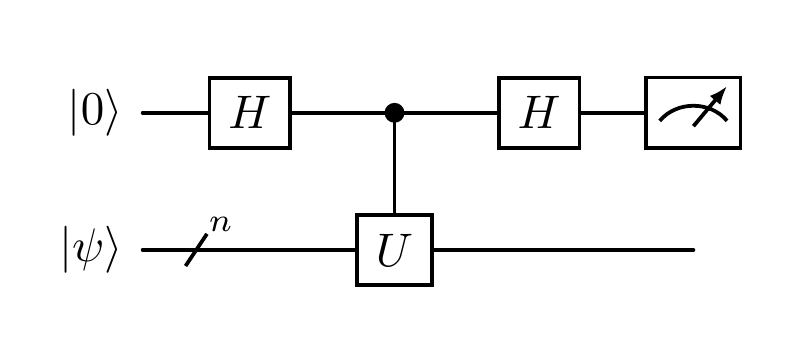
\begin{tikzpicture}
\node[scale=1.7]{
\begin{quantikz}
\lstick{$\ket{0}$}    & \gate{H}     & \ctrl{1} & \gate{H} & \meter{} \\    
\lstick{$\ket{\psi}$} & \qwbundle{n} & \gate{U} &          &  
\end{quantikz}
};
\end{tikzpicture}
\end{align}
Jeśli zmierzymy na wyjściu $\ket{0}$ to wypluwamy $1$. Jeśli zmierzymy $\ket{1}$ to wypluwamy $-1$. \\
Wtedy wartość oczekiwana na wyjściu jest równa dokładnie $\Re \bra{\psi}U\ket{\psi}$.
\begin{proof}
    Przeanalizujmy co się kolejno dzieje w naszym układzie. \\
    Na wejściu mamy stan $\ket{0}\ket{\psi}$. Aplikujemy na górnym kablu Hadamarda, który działał tak:
    \[ H\ket{0} = \frac{1}{\sqrt2}\Bigl( \ket{0}+\ket{1} \Bigr), \qquad H\ket{1} = \frac{1}{\sqrt2}\Bigl( \ket{0}-\ket{1} \Bigr) \]
    Czyli u nas:
    \[ \ket{0}\ket{\psi} \xmapsto{H\otimes I_n} \frac{1}{\sqrt2}\Bigl( \ket{0}+\ket{1} \Bigr) \otimes \ket{\psi} \]
    Bramka $U$ jest kontrolowana, czyli aplikuje się tylko dla $\ket{1}$ na kontrolującym kubicie:
    \[ \frac{1}{\sqrt2}\Bigl( \ket{0}+\ket{1} \Bigr) \otimes \ket{\psi} \xmapsto{CU} \frac{1}{\sqrt2}\Bigl( \ket{0}\otimes \ket{\psi}+\ket{1}\otimes U\ket{\psi} \Bigr)  \] 
    Na końcu znowu aplikujemy Hadamarda:
    \[ \frac{1}{\sqrt2}\Bigl( \ket{0}\otimes \ket{\psi}+\ket{1}\otimes U\ket{\psi} \Bigr) \xmapsto{H\otimes I_n} \frac{1}{2}\Bigl( \left( \ket{0}+\ket{1} \right)\otimes \ket{\psi}+\left( \ket{0}-\ket{1} \right)\otimes U\ket{\psi} \Bigr) = \]
    \[ = \frac{1}{2}\Bigl( \ket{0}\otimes \left( \ket{\psi}+U\ket{\psi} \right) + \ket{1}\otimes \left( \ket{\psi}-U\ket{\psi} \right) \Bigr) \]
    \[ = \frac{1}{2}\Bigl( \ket{0}\otimes \left( I+U \right)\ket{\psi} + \ket{1}\otimes \left( I-U \right)\ket{\psi} \Bigr) \]
    Świetnie, zatem prawdopodobieństwo otrzymania $\ket{0}$ to kwadrat ze współczynnika przy nim swojącego. W ogólności jeśli stoi tam wektor stanów $\ket{\phi}$ to prawdopodobieństwo wynosi $\braket{\phi}{\phi} = \ket{\phi}^\dagger \ket{\phi}$. Zatem liczymy prawdopodobieństwo $p_0$ zmierzenia $\ket{0}$:
    \[ p_0 = \frac{1}{4}\left(\left( I+U \right)\ket{\psi}\right)^\dagger\left( I+U \right)\ket{\psi}
    = \frac{1}{4}\bra{\psi}\left( I+U^\dagger\right)\left( I+U \right)\ket{\psi} \]
    Jeśli powtórzymy analogiczne rozumowanie do policzenia prawdopodobieństwa $p_1$ zmierzenia na wyjściu $\ket{1}$ to otrzymamy, że:
    \[ p_1 = \frac{1}{4}\bra{\psi}\left( I-U^\dagger\right)\left( I-U \right)\ket{\psi} \] \\
    I teraz gwóźdź programu: traktujemy każde zmierzone $\ket{0}$ jako $1$, a każde $\ket{1}$ jako $-1$. Oznaczmy tą zmienną losową przez $X$. Z definicji wartości oczekiwanej mamy: 
    \[ E[X] = p_0\cdot (1) + p_1\cdot(-1) \]
    \[ = \frac{1}{4}\bra{\psi}\Bigl[\left( I+U^\dagger\right)\left( I+U \right) - \left( I-U^\dagger\right)\left( I-U \right)\Bigr]\ket{\psi} \]
    \[ = \frac{1}{4}\bra{\psi}\Bigl[ \ccancel[red]{\,I\,}+U+U^\dagger+\ccancel[red]{U^\dagger U}-\ccancel[red]{\,I\,}+U+U^\dagger-\ccancel[red]{U^\dagger U}  \Bigr]\ket{\psi}  \]
    \[ = \frac{1}{2}\bra{\psi}\Bigl( U + U^\dagger \Bigr)\ket{\psi} \enspace = \enspace \frac{1}{2}\bra{\psi}U\ket{\psi} + \frac{1}{2}\Bigl(\bra{\psi}U\ket{\psi}\Bigr)^\dagger \] \\
    Ale zauważmy, że $\bra{\psi}U\ket{\psi} = z\in \C$. Zatem $\Bigl(\bra{\psi}U\ket{\psi}\Bigr)^\dagger = z^\dagger = \bar{z}$. Ale z własności liczb zespolonych mamy, że $z+\bar{z} = 2\Re z$. Zatem:
    \[ E[X] = \frac{1}{2}(z+\bar{z}) = \Re z \]

\end{proof}
Co jednak, jeśli chcielibyśmy zmierzyć wartość $\Im \bra{\psi}U\ket{\psi}$? Okazuje się, że możemy tego dokonać w analogiczny sposób, nieznacznie modyfikując układ:
\begin{align}
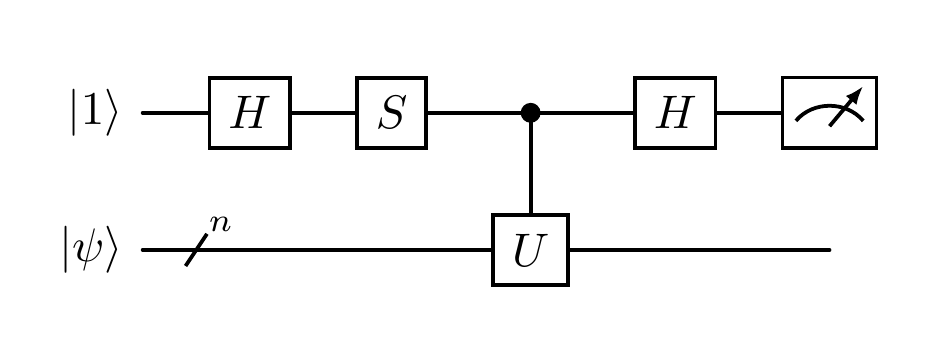
\begin{tikzpicture}
\node[scale=1.7]{
\begin{quantikz}
\lstick{$\ket{1}$}    & \gate{H}     & \gate{S}  & \ctrl{1} & \gate{H} & \meter{} \\    
\lstick{$\ket{\psi}$} & \qwbundle{n} &           & \gate{U} &          &  
\end{quantikz}
};
\end{tikzpicture}
\end{align}

gdzie \( S = \mat{1, 0}{0, i} \) - \textit{Phase gate}. Działa ona w następujący sposób:
\[ S\ket{0} = \ket{0},\quad S\ket{1} = i\ket{1} \]
Otrzymujemy zatem:
\[ \ket{1}\ket{\psi} \xmapsto{H\otimes I} \frac{1}{\sqrt2}\Bigl(\ket{0}-\ket{1}\Bigr)\ket{\psi} \xmapsto{S\otimes I} \frac{1}{\sqrt2}\Bigl(\ket{0}-i\ket{1}\Bigr)\ket{\psi} \]
Teraz postępujemy analogicznie jak wcześniej:
\[ \xmapsto{CU} \frac{1}{\sqrt2}\Bigl(\ket{0}-i\ket{1}U\Bigr)\ket{\psi} \]
\[ \xmapsto{H\otimes I} \dots = \frac{1}{\sqrt2}\left[\ket{0}\Bigl(\ket{\psi}-iU\ket{\psi}\Bigr) + \ket{1}\Bigl(\ket{\psi}+iU\ket{\psi}\Bigr)\right] \]
Prawdopodobieństwo zmierzenia $0$:
\[ p_0 = \frac{1}{4}\Bigl(\ket{\psi}-iU\ket{\psi}\Bigr)^\dagger\Bigl(\ket{\psi}-iU\ket{\psi}\Bigr)
       = \frac{1}{4}\Bigl(\bra{\psi}+iU^\dagger\bra{\psi}\Bigr)\Bigl(\ket{\psi}-iU\ket{\psi}\Bigr) \]
\[ = \frac{1}{4}\bra{\psi}\Bigl(I+iU^\dagger\Bigr)\Bigl(I-iU\Bigr)\ket{\psi} \]
Powtarzając to samo rozumowanie jak dla standardowej wersji testu i pamiętając, że dla $z\in \C$ mamy $(-iz) + (\overline{-iz}) = 2\Im z$ dostaniemy, że układ faktycznie w oczekiwaniu wypluwa $\Im z$. 
\subsection{Test SWAP}

\begin{problem*}{}{}
    Dane są dwa stany $\ket{\phi}$ oraz $\ket{\psi}$. Zadaniem naszym jest oszacowanie wartości $|\braket{\phi}{\psi}|^2$.
\end{problem*}
Zauważmy, że test SWAP osiąga cel podobny do testu Hadamarda - pozwala nam ocenić, jak bardzo ''podobne'' są do siebie dwa stany $\ket{\phi}$ i $\ket{\psi}$. \\
Sam układ wygląda tak:
\begin{align}
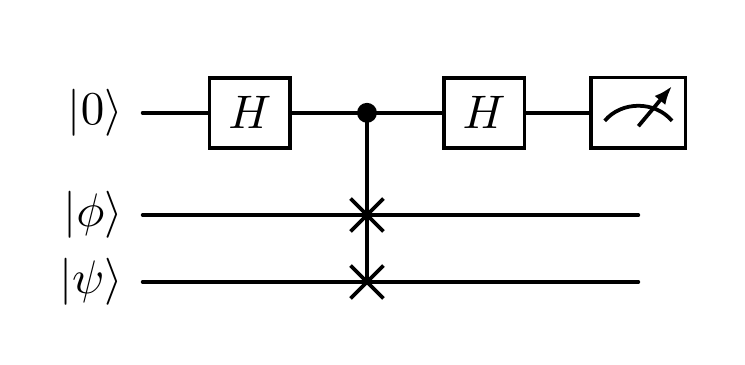
\begin{tikzpicture}
\node[scale=1.7]{
\begin{quantikz}
\lstick{$\ket{0}$}    & \gate{H} & \ctrl{1} & \gate{H} & \meter{} \\    
\lstick{$\ket{\phi}$} &          & \swap{1} &          &          \\
\lstick{$\ket{\psi}$} &          & \targX{} &          &  
\end{quantikz}
};
\end{tikzpicture}
\end{align}
Główna bramka w nim występująca to kontrolowana bramka SWAP, która zamienia dwa dolne wejścia miejscami jeśli dostanie $\ket{1}$ na górnym kablu. \\ 
Jeśli każde zmierzone $\ket{0}$ potraktujemy jako $1$, a każde $\ket{1}$ jako $-1$, to okaże się, że wartość oczekiwana takiej zmiennej losowej wynosi $|\braket{\phi}{\psi}|^2$.
\begin{proof}
    Prześledźmy kolejne aplikacje bramek w naszym układzie:
    \[ \ket{0\phi\psi} \xmapsto{H \otimes I \otimes I} \frac{1}{\sqrt2} \Bigl(\ket{0\phi\psi} + \ket{1\phi\psi} \Bigr)
     \xmapsto{CSWAP} \frac{1}{\sqrt2} \Bigl(\ket{0\phi\psi} + \ket{1\psi\phi} \Bigr) \]
    \[ \xmapsto{X\otimes I \otimes I} \frac{1}{2} \Bigl(\bigl(\ket{0}+\ket{1}\bigr)\ket{\phi\psi} + \bigl(\ket{0}-\ket{1}\bigr)\ket{\psi\phi} \Bigr)
      =  \frac{1}{2}\ket{0}\bigl(\ket{\phi\psi} + \ket{\psi\phi}\bigr) + \frac{1}{2}\ket{1}\bigl(\ket{\phi\psi} - \ket{\psi\phi}\bigr) \] \\
    Liczymy prawdopodobieństwo $p_0$ uzyskania $\ket{0}$:
    \[ p_0 = \frac{1}{4}\Bigl(\ket{\phi\psi} + \ket{\psi\phi}\Bigr)^\dagger \Bigl(\ket{\phi\psi} + \ket{\psi\phi}\Bigr)
        = \frac{1}{4}\Bigl(\bra{\psi\phi} + \bra{\phi\psi}\Bigr)\Bigl(\ket{\phi\psi} + \ket{\psi\phi}\Bigr) \]
    \[ = \frac{1}{4} \Bigl( \braket{\psi\phi}{\phi\psi} + \braket{\psi\phi}{\psi\phi} + \braket{\phi\psi}{\phi\psi} +  \braket{\phi\psi}{\psi\phi} \Bigr) \]
    \[ = \frac{1}{4} \Bigl( 1 + \left|\braket{\phi}{\psi}\right|^2 + \left|\braket{\phi}{\psi}\right|^2 + 1 \Bigr) \]
    \[ = \frac{1}{2} + \frac{1}{2}\left|\braket{\phi}{\psi}\right|^2 \]

    gdzie $\braket{\psi\phi}{\psi\phi} = \braket{\phi\psi}{\phi\psi} = \left| \braket{\phi}{\psi} \right|^2$ bierze się stąd:
    \[ \braket{\psi\phi}{\psi\phi} = \bra{\psi}\underbrace{\bra{\phi}\ket{\psi}}_\textrm{$\in\C$}\ket{\phi} = \braket{\psi}{\phi}\braket{\phi}{\psi} = \Bigl(\braket{\phi}{\psi}\Bigr)^\dagger \braket{\phi}{\psi} = \left|\braket{\phi}{\psi}\right|^2 \]
    Z tego mamy, że prawdopodobieństwa $p_1$ otrzymania $\ket{1}$:
    \[ p_1 = \frac{1}{2} - \frac{1}{2} \left|\braket{\phi}{\psi}\right|^2\]
    Wprowadźmy teraz naszą zmienną losową $X$. Z prawdopodobieństwem $p_0$ otrzymujemy 1, a z prawd. $p_1$ dostajemy $-1$. Pozostaje wyznaczyć $E[X]$:
    \[ E[X] = p_0 \cdot (1) + p_1 \cdot (-1) 
       = \ccancel[red]{\,\frac{1}{2}\,} + \frac{1}{2}\left|\braket{\phi}{\psi}\right|^2 - \ccancel[red]{\,\frac{1}{2}\,} + \frac{1}{2} \left|\braket{\phi}{\psi}\right|^2 
       = \left|\braket{\phi}{\psi}\right|^2 \]
\end{proof}
\begin{lemma*}{}
Dla ustalonej prezycji $\varepsilon$ zarówno test Hadamarda jak i test SWAP wymagają $N = \Os(1/\varepsilon^2)$ prób.
\end{lemma*}

\begin{proof}
    Bierze się to z faktu, że oba $N$ razy próbkują pewną zmienną losową, która zwraca jeden z możliwych wyników ze stałym prawdopodobieństwem $p$. Dla pojedynczej próby $X_i$ wariancja $Var[X_i]$ jest stała, tj. $Var[X_i]=\Os(1)$. Każda próba jest niezależna od pozostałych, czyli dla $X=\frac{1}{N}\bigl(X_1+\dots+X_N\bigr)$ mamy:
    \[Var[X] = Var\left[\frac{1}{N}\Bigl(X_1+\dots+X_N\Bigr)\right] = \frac{1}{N^2}Var[X_1+\dots+X_N] = \frac{1}{N^2}\sum_{i=1}^{N}Var[X_i]= \frac{1}{N^2}\Os(N) = \Os\left(\frac{1}{N}\right) \]   
A odchylenie standardowe $\sigma(X) = \sqrt{Var[X]} = \Os\left(\frac{1}{\sqrt{N}}\right)$. Czyli chcąc $\sigma(X) \le \varepsilon$ potrzebujemy:
\[ \sigma(X) \le \varepsilon \enspace \iff* \enspace \Os\left(\frac{1}{\sqrt{N}}\right) \le \varepsilon \enspace \iff* \enspace \Os\left(\frac{1}{N}\right) \le \varepsilon^2 \enspace \iff* N = \Os\left(\frac{1}{\varepsilon^2}\right)\] \\
\end{proof}

% ------------------------------------------------------------------------------------------
\newpage
\section{Stabilizatory}
\begin{definition*}{}
    Wyróżniamy cztery \textbf{bramki Pauliego}:
    \[ X = \mat{0,1}{1,0},\quad Y = \mat{0,-i}{i,0},\quad Z = \mat{1,0}{0,-1},\quad I = \mat{1,0}{0,1} \]
\end{definition*}
Zwane są też po prostu macierzami Pauliego. Mają parę ciekawych własności.
\begin{itemize}
    \item Dwie różne bramki Pauliego, niebędące $I$, \textit{antykomutują}, czyli:
\[ XY = -YX,\enspace XZ = -ZX,\enspace YZ = -ZY \]
    \item Każda jest własną odwrotnością:
        \[ X^2 = Y^2 = Z^2 = I \]
    \item Ogólnie to z dokładnością do fazy tworzą zamkniętą grupę:
        \[ XY = iZ \qquad YX = -iZ \] 
        \[ YZ = iX \qquad ZY = -iX \] 
        \[ ZX = iY \qquad XZ = -iY \]
    \item Wszystkie są unitarne i hermitowskie. 

\end{itemize}

\begin{definition*}{}
    \textbf{Grupą Pauliego} dla pojedynczego kubitu nazywamy grupę
    \[ P_1 = \{\pm 1,\pm i\}\times \{X,Y,Z,I\} \]
    Definicja działa również dla większej ilości kubitów:  
    \[ P_n = \{\pm 1,\pm i\}\times \{X,Y,Z,I\}^{\otimes n} \]
\end{definition*}
\begin{definition*}{}
    Mówimy, że operator unitarny $U$ \textbf{stabilizuje} stan $\ket{\psi}$, jeśli $U\ket{\psi} = \ket{\psi}$. \\
    Wtedy $U$ nazywamy \textbf{stabilizatorem}. \\
    Równoważnie można powiedzieć, że stan $\ket{\psi}$ jest \textbf{stabilizowany} przez operator $U$.
\end{definition*}
\begin{definition*}{}
    Niech $\ket{\psi}$ to dowolny (określony) stan $n$-kubitowy. \\
    Wtedy \textbf{grupa stabilizująca} $G$ to podzbiór wszystkich $P_n$ stabilizujących $\ket{\psi}$.  
\end{definition*}
Mają one ciekawe własności. Załóżmy, że mamy grupę stabilizujacą $G\le P_n$ na $n$ kubitach. Wtedy:
\begin{itemize}
    \item $G$ jest abelowa ($PQ\in G \iff* QP\in G$)
    \item $-I^{\otimes n} \notin G$
\end{itemize}  

\begin{definition*}{}
    \textbf{Wymiar} grupy $G$ definiujemy następująco:
        \[ \dim(G) := \log_2|G| \]
    Równoważnie wymiar to ilość generatorów danej grupy. 
\end{definition*}
W szczególności $\dim(G)=k\in \N$ jest równoważne temu, że $|G|=2^k$. \\
Ale przecież jeśli $G\le P_n$, to z tw. Lagrange'a mamy, że $|G|$ dzieli $|P_n|$. Ale (z definicji) $P_n=4^{n+1}$. Oznacza to, że zawsze $G=2^k$, dla pewnego $k\in \N$. \\

\begin{definition*}{}
    \textbf{Bramką Clifforda} nazywamy bramkę kwantową $U$, dla której zachodzi:
    \[ UPU^{-1}\in P_n \]
    dla każdego $P\in P_n$.
\end{definition*}
\begin{examples}{\,} \\
    \begin{itemize}
        \item Bramka Hadamarda - \textcolor{green}{\ding{51}} \\
            Jest tak, gdyż:
            \[ HXH^\dagger = Z, \quad HYH^\dagger = -Y, \quad HZH^\dagger = X \]
            A wszystkie wynikowe bramki oczwiście są Pauliego, czyli z definicji $H$ jest bramką Clifforda.
        \item Bramka S - \textcolor{green}{\ding{51}} \\
            Przypomnijmy, że $S = \mat{1, 0}{0, i}$. Wtedy:
            \[ SXS^\dagger = Y, \quad SYS^\dagger = -X, \quad SZS^\dagger = Z \]
        \item Bramka T - \textcolor{red}{\ding{55}} \\
            Przypomnijmy, że $T = P(\pi/4) = \mat{1, 0}{0, e^{i\frac{\pi}{4}}}$. Ale mamy, że:
            \[ TXT^\dagger = \mat{1, 0}{0, \frac{1+i}{\sqrt2}} \cdot \mat{0, 1}{1, 0} \cdot \mat{1, 0}{0, \frac{1-i}{\sqrt2}}
                           = \mat{0, 1}{\frac{1+i}{\sqrt2}, 0} \cdot \mat{1, 0}{0, \frac{1-i}{\sqrt2}}
                           = \mat{0, \frac{1-i}{\sqrt2}}{\frac{1+i}{\sqrt2}, 0} \]
            Ale nie jest to żadna z bramek Pauliego, więc $T$ nie jest bramką Clifforda.
    \end{itemize}
\end{examples}
\begin{fact}{\textbf{(1)}}
    $Cliff_n = \langle H, S, CX \rangle$.
\end{fact}
Gdzie zapis $\langle\dots\rangle$ oznacza grupę/zbiór generowane przez zadane bramki.
\begin{fact}{\textbf{(2)}}
    Zbiór bramek $Cliff + T$ jest \textit{uniwersalny}
\end{fact}

\begin{theorem*}{(Gotessman-Knill)}
    Obwody kwantowe złożone tylko z bramek Clifforda da się wielomianowo zasymulować na klasycznym komputerze.
\end{theorem*}

% ------------------------------------------------------------------------------------------

\newpage
\section{Adiabatic QC}
Na dzień dzisiejszy nie jesteśmy w stanie zaimplementować nawet prostych algorytmów kwantowych. A o Shorze czy Groverze to możemy zapomnieć. Problemem są błędy obliczeń, dekoherencja czy po prostu za mała liczba kubitów w systemach. \\
Nie wszystko jednak stracone, bo istnieją już \textit{prawie} praktyczne algorytmy kwantowe służące do rozwiązywania zadań optymalizacyjnych. Działają one na trochę innej zasadzie niż te, z którymi się spotkaliśmy wcześniej. Z tego powodu wyróżnia się to inne podejście jako osobny paradygmat \textit{adiabatycznych} obliczeń kwantowych (adiabatic QC).  
\begin{theorem*}{(Variational Principle)}
    Niech $H$ będzie znanym nam (niezależnym od czasu) Hamiltonianem. Niech $\ket{\psi}$ reprezentuje pewien stan kwantowy. Wtedy energię $E_\psi$ stanu $\ket{\psi}$ wyliczamy następująco:
    \[ E_\psi = \bra{\psi}H\ket{\psi} \]
    Niech $E_0$ określa najmniejszą możliwą energię, osiąganą dla pewnego stanu bazowego. \\
    \textbf{Variational Principle} mówi po prostu, że:
    \[ E_0 \le \bra{\psi}H\ket{\psi} \]
\end{theorem*} 



\begin{definition*}{(Barren plateaus)}
Mianem \textbf{Barren plateaus} określamy zjawisko występowania nieproporcjonalnie dużych, (wykładniczo) płaskich regionów funkcji kosztu w kwantowych problemach optymalizacyjnych. 
\end{definition*}
Fakt występowania tych równin jest o tyle niefortunny, że niepraktyczne staje się stosowanie tradycyjnego spadku wzdłuż gradientu. Niepraktyczne, bo gradient ten jest prawie zawsze równy 0, i algorytm nie jest w stanie znaleźć minimum. Duża część obecnych skupia się na tym by zrozumieć i przeciwdziałać fenomenowi równin Barrena.   

% ------------------------------------------------------------------------------------------
% \newpage
% \section{Zastosowania}
% \begin{definition*}{(Electronic Hamiltonian)}
%     \[ \hat{H}^{(el.)} = \sum_{ij\sigma}h_{ij}a_{i\sigma}^\dagger a_{j\sigma} + \sum_{ijk\sigma kl\tau}g_{ijkl}+a_{i\sigma}^\dagger a_{j\sigma}a_{k\tau}^\dagger a_{l\tau} \]
%     gdzie:
%     \begin{itemize}
%         \item $\sigma \in \{\uparrow,\downarrow\}$ - spin index
%         \item $p \in \{\uparrow,\downarrow\}$ - orbital index
%         \item $\delta_{ij} = [i=j]$ - delta Diraca
%         \item $a$ oraz $a_\dagger$ to \textit{creation / anihillation operators}, czyli:
%         \[ a^\dagger\ket{0} = \ket{1} \] 
%         \[ a\ket{0} = \ket{0}, \quad a\ket{1} = \ket{0} \] 

%     \end{itemize}
% \end{definition*}
% Muszą zachodzić takowe własności:
% \[ \left[\hat{a}^\dagger_{p\sigma}, \hat{a}_{q\rho}\right]_+  = TODO \]
% \begin{fact}
%     Dla $\ket{n_1,\dots,n_N}, n_k\in\{0,1\}$ zachodzi:
%     \[ a_k^+\ket{n_1,\dots,n_N} = (-1)^{\sum_{j<k}n_j}\ket{n_1,\dots,n_k+1,\dots,n_N} \]
% \end{fact}
% \begin{definition*}{(Transformacja Jordana-Wignera)}
%     \[ \hat{a}_{p\sigma} = \hat{a}_{\sigma N+p} = TODO \]
%     gdzie:
%     \begin{itemize}
%         \item $\sigma_k^+$ - creation operator, zdefiniowany jako $\sigma_k^+ = \frac{1}{2}\left(X_k-iY_k\right)$
%     \end{itemize}
% \end{definition*}

% $U(t) = exp(-i\hat{H}t/\lambda)\approx f(\frac{\hat{H}t}{\lambda})$

\end{document}